\section{Theoretical Supplement}
\label{app:theory}

\subsection{HT-MG-BC Formal Setting}
\label{sec:setting-app}

\paragraph{Heterogeneous-Type Markov Game.}
An HT-MG is a tuple
$\mathcal{G} = \langle \mathcal{S}, \{\mathcal{A}_i\}, P^*, \{\Theta_i\}, \{r_i\}, P_0, H \rangle$
with finite state space $|\mathcal S|=S$, joint action space $\mathcal A=\prod_i \mathcal A_i$ of size $A_{\mathrm{joint}}$, type space $\Theta=\prod_i \Theta_i$, transition kernel $P^*\!:\!\mathcal S\!\times\!\mathcal A\!\times\!\Theta\to\Delta(\mathcal S)$, per-agent reward $r_i\!:\!\mathcal S\!\times\!\mathcal A\!\times\!\Theta_i\!\to\![0,1]$, joint prior $P_0$, and horizon $H$. At the start of each episode a type profile $\boldsymbol\theta^* \in \Theta$ is sampled once and held fixed; $P^*$ is fixed across episodes but unknown. A centralised learner observes the full trajectory $\tau_k$ and updates a posterior over $(P^*, \boldsymbol\theta^*)$.

\paragraph{Structural assumptions.} The decoupling theorem rests on three:
(\textbf{TI}, Assumption~\ref{ass:TI}) the transition kernel does not depend on the type profile;
(\textbf{RL}, Assumption~\ref{ass:RL}) each $r_i$ depends only on $\theta_i$ (other agents' actions $a_{-i}$ may still influence reward);
(\textbf{PF}, Assumption~\ref{ass:PF}) the prior factorises as $P_0(P,\boldsymbol\theta)=P_0^P(P)\prod_i P_0^{\Theta,i}(\theta_i)$.
The regret analysis additionally uses type-identifiability (\textbf{TID}, Assumption~\ref{ass:TID}: per-step Hellinger gap $\geq\rho$), initial-state independence (\textbf{ISI}, Assumption~\ref{ass:ISI}), and a deterministic CCE selection rule (\textbf{CSR}, Assumption~\ref{ass:CSR}). Both TI and RL are individually necessary: violating either breaks the likelihood factorisation, as shown by two counter-examples in Appendix~\ref{sec:necessity}.

\begin{assumption}[TI]\label{ass:TI}$P^*(s'\!\mid\! s,a,\boldsymbol\theta)=P^*(s'\!\mid\! s,a)$.\end{assumption}
\begin{assumption}[RL]\label{ass:RL}$r_i(s,a,\boldsymbol\theta)=r_i(s,a,\theta_i)$.\end{assumption}
\begin{assumption}[PF]\label{ass:PF}$P_0(P,\boldsymbol\theta)=P_0^P(P)\prod_i P_0^{\Theta,i}(\theta_i)$.\end{assumption}
\begin{assumption}[TID]\label{ass:TID}$\inf_{s,a}D_H^2(P(\cdot\!\mid\! s,a,\theta_i),P(\cdot\!\mid\! s,a,\theta_i'))\geq\rho>0$ for all $\theta_i\!\neq\!\theta_i'$.\end{assumption}
\begin{assumption}[ISI]\label{ass:ISI}$s_1^k\sim\beta$ fixed and independent of $(P^*,\boldsymbol\theta^*)$.\end{assumption}
\begin{assumption}[CSR]\label{ass:CSR}$\mathrm{CCE}(\cdot,\cdot)$ is a measurable deterministic mapping.\end{assumption}

\paragraph{Performance criterion.} Let $\pi^{\mathrm{CCE}}(P,\boldsymbol\theta)$ denote a CCE policy of the MG induced by $(P,\boldsymbol\theta)$. The type-conditional Bayesian regret of agent $i$ over $K$ episodes is
\begin{equation}\label{eq:regret-def}\resizebox{0.9\linewidth}{!}{$\displaystyle \mathrm{Reg}_i^B(K) \!\coloneqq\! \mathbb{E}_{(P^*,\boldsymbol\theta^*)\sim P_0}\!\sum_{k=1}^K\!\Big(V_i^{\pi^{\mathrm{CCE}}(P^*,\boldsymbol\theta^*)}\!(s_1^k;\theta_i^*) - V_i^{\pi_k}(s_1^k;\theta_i^*)\Big). $}\end{equation}

\subsection{Posterior Decoupling Theorem}
\label{sec:decoupling}

This section states and proves the main structural result.

\subsubsection{Likelihood Factorization}

We first derive the conditional likelihood of an observed trajectory given the latent world. Under PACT, the policy $\pi_k$ at episode $k$ is a function only of the history $\mathcal{H}_{k-1}$ and the algorithmic posterior samples $(\hat{P}_k, \hat{\boldsymbol{\theta}}_k)$, which are themselves measurable with respect to $\mathcal{H}_{k-1}$. Crucially, $\pi_k$ does not depend on the true latent $(P^*, \boldsymbol{\theta}^*)$.

\begin{lemma}[Joint Likelihood Factorization]
\label{lem:likelihood}
Under Assumptions~\ref{ass:TI} and \ref{ass:RL}, the trajectory likelihood at episode $k$ factorizes as
\begin{equation}\label{eq:lik-factor}\resizebox{0.9\linewidth}{!}{$\displaystyle P(\tau_k \mid P, \boldsymbol{\theta}, \mathcal{H}_{k-1}) = c_k(\tau_k) \cdot L_P(\tau_k; P) \cdot \prod_{i \in [n]} L_{\Theta,i}(\tau_k; \theta_i) $}\end{equation}
where
\begin{align}
c_k(\tau_k) &:= \mathbb{E}_{\pi_k \mid \mathcal{H}_{k-1}}\left[\prod_{h=1}^H \pi_k(a_h^k \mid s_h^k)\right], \label{eq:ck} \\
L_P(\tau_k; P) &:= \prod_{h=1}^H P(s_{h+1}^k \mid s_h^k, a_h^k), \label{eq:lp} \\
L_{\Theta,i}(\tau_k; \theta_i) &:= \prod_{h=1}^H P(r_h^{k,i} \mid s_h^k, a_h^k, \theta_i). \label{eq:ltheta}
\end{align}
The constant $c_k(\tau_k)$ depends on $\tau_k$ and $\mathcal{H}_{k-1}$ but not on $(P, \boldsymbol{\theta})$.
\end{lemma}

\begin{proof}
Conditional on $\pi_k$, the trajectory likelihood unrolls along the time axis as
\begin{equation}\resizebox{0.9\linewidth}{!}{$\displaystyle P(\tau_k \mid \pi_k, P, \boldsymbol{\theta}) = \prod_{h=1}^H \pi_k(a_h^k \mid s_h^k) \cdot P(s_{h+1}^k \mid s_h^k, a_h^k, \boldsymbol{\theta}) \cdot \prod_{i \in [n]} P(r_h^{k,i} \mid s_h^k, a_h^k, \boldsymbol{\theta}). $}\end{equation}
Apply Assumption~\ref{ass:TI} to drop $\boldsymbol{\theta}$ from the transition factor, and Assumption~\ref{ass:RL} to localize the reward factor to $\theta_i$:
\begin{equation}\resizebox{0.9\linewidth}{!}{$\displaystyle P(\tau_k \mid \pi_k, P, \boldsymbol{\theta}) = \prod_{h=1}^H \pi_k(a_h^k \mid s_h^k) \cdot \prod_{h=1}^H P(s_{h+1}^k \mid s_h^k, a_h^k) \cdot \prod_{h=1}^H \prod_{i \in [n]} P(r_h^{k,i} \mid s_h^k, a_h^k, \theta_i). $}\end{equation}
Marginalize over $\pi_k$ with respect to $P(\pi_k \mid \mathcal{H}_{k-1})$, which is independent of $(P, \boldsymbol{\theta})$:
\[\resizebox{\linewidth}{!}{$\displaystyle\begin{aligned}
P(\tau_k \mid P, \boldsymbol{\theta}, \mathcal{H}_{k-1}) &= \int P(\pi_k \mid \mathcal{H}_{k-1}) \cdot P(\tau_k \mid \pi_k, P, \boldsymbol{\theta}) \, d\pi_k \\
&= \mathbb{E}_{\pi_k \mid \mathcal{H}_{k-1}}\left[\prod_{h=1}^H \pi_k(a_h^k \mid s_h^k)\right] \cdot L_P(\tau_k; P) \cdot \prod_{i \in [n]} L_{\Theta,i}(\tau_k; \theta_i).
\end{aligned}$}\]
The factors $L_P$ and $L_{\Theta,i}$ depend respectively on $P$ alone and $\theta_i$ alone, and the leading expectation depends on $\tau_k$ and $\mathcal{H}_{k-1}$ alone.
\end{proof}

\subsubsection{Main Theorem}

\begin{theorem}[Posterior Decoupling]
\label{thm:decoupling-app}
Under Assumptions~\ref{ass:TI}, \ref{ass:RL}, and \ref{ass:PF}, the posterior distribution over the latent world factorizes at every episode:
\begin{equation}\label{eq:decoupling-app}\resizebox{0.9\linewidth}{!}{$\displaystyle P(P, \boldsymbol{\theta} \mid \mathcal{H}_k) = \mu_{k+1}^P(P) \cdot \prod_{i \in [n]} \mu_{k+1}^{\Theta,i}(\theta_i), \quad \forall k \in \{0, 1, \ldots, K\} $}\end{equation}
where the marginals admit the recursive updates
\begin{equation}\resizebox{0.9\linewidth}{!}{$\displaystyle \mu_{k+1}^P(P) \propto \mu_k^P(P) \cdot L_P(\tau_k; P), \quad \mu_{k+1}^{\Theta,i}(\theta_i) \propto \mu_k^{\Theta,i}(\theta_i) \cdot L_{\Theta,i}(\tau_k; \theta_i) $}\end{equation}
with initial conditions $\mu_1^P = P_0^P$ and $\mu_1^{\Theta,i} = P_0^{\Theta,i}$.
\end{theorem}

\begin{proof}
We proceed by induction on $k$.

\textit{Base case ($k=0$).} By Assumption~\ref{ass:PF}, $P(P, \boldsymbol{\theta} \mid \mathcal{H}_0) = P_0(P, \boldsymbol{\theta}) = P_0^P(P) \prod_{i \in [n]} P_0^{\Theta,i}(\theta_i)$, which has the required factored form.

\textit{Inductive step.} Suppose $P(P, \boldsymbol{\theta} \mid \mathcal{H}_{k-1}) = \mu_k^P(P) \prod_{i} \mu_k^{\Theta,i}(\theta_i)$. By Bayes' rule,
\begin{equation}\resizebox{0.9\linewidth}{!}{$\displaystyle P(P, \boldsymbol{\theta} \mid \mathcal{H}_k) \propto P(P, \boldsymbol{\theta} \mid \mathcal{H}_{k-1}) \cdot P(\tau_k \mid P, \boldsymbol{\theta}, \mathcal{H}_{k-1}). $}\end{equation}
Apply Lemma~\ref{lem:likelihood}:
\[\resizebox{\linewidth}{!}{$\displaystyle\begin{aligned}
P(P, \boldsymbol{\theta} \mid \mathcal{H}_k) &\propto \mu_k^P(P) \prod_{i} \mu_k^{\Theta,i}(\theta_i) \cdot c_k(\tau_k) \cdot L_P(\tau_k; P) \cdot \prod_{i} L_{\Theta,i}(\tau_k; \theta_i) \\
&\propto \left[\mu_k^P(P) L_P(\tau_k; P)\right] \cdot \prod_{i} \left[\mu_k^{\Theta,i}(\theta_i) L_{\Theta,i}(\tau_k; \theta_i)\right].
\end{aligned}$}\]
The factor $c_k(\tau_k)$ does not depend on $(P, \boldsymbol{\theta})$ and is absorbed into the normalization constant. The remaining product factorizes into a $P$-only term and $n$ separate $\theta_i$-only terms. Normalizing each factor independently yields the recursive forms stated in the theorem and establishes the desired posterior factorization.
\end{proof}

\begin{corollary}[Storage and Update Complexity]
\label{cor:storage}
Maintaining the joint posterior $P(P, \boldsymbol{\theta} \mid \mathcal{H}_k)$ under PACT requires $O\left(\dim(P_0^P) + n |\Theta|\right)$ storage, as opposed to the naive $O\left(\dim(P_0^P) \cdot |\Theta|^n\right)$ that a non-factored posterior would require. Each Bayesian update costs $O(H)$ likelihood evaluations per module.
\end{corollary}

\begin{proposition}[Trajectory-Level Equivalence with Joint-PSRL]
\label{prop:bit-identical}
Consider an idealised Joint-PSRL algorithm that maintains the joint posterior $\mu_k^\Theta$ on $\Theta = \prod_i \Theta_i$ and at each episode samples $\hat{\boldsymbol\theta}_k \sim \mu_k^\Theta$. Under the assumptions of Theorem~\ref{thm:decoupling-app} and \emph{coupled RNG} (formalised below), the trajectories produced by PACT and Joint-PSRL are pathwise identical: $\tau_k^{\mathrm{H\text{-}PSMG}} = \tau_k^{\mathrm{Joint\text{-}PSRL}}$ for every $k \geq 1$ almost surely. In particular the cumulative regrets agree exactly:
\begin{equation}\resizebox{0.9\linewidth}{!}{$\displaystyle \mathrm{Reg}_i^B\big[\textnormal{PACT}\big](K) = \mathrm{Reg}_i^B\big[\textnormal{Joint-PSRL}\big](K) \quad \forall i, K, \text{ a.s.} $}\end{equation}

The coupling is constructed as follows. At episode $k$, both algorithms draw a single shared seed $u_k = (u_k^P, u_k^{\Theta, 1}, \ldots, u_k^{\Theta, n}) \sim \mathrm{Unif}([0,1]^{n+1})$. PACT uses $u_k^P$ to sample $\hat P_k = F_{\mu_k^P}^{-1}(u_k^P)$ and $u_k^{\Theta, i}$ to sample $\hat\theta_i^k = F_{\mu_k^{\Theta, i}}^{-1}(u_k^{\Theta, i})$ via the inverse-CDF transform. Joint-PSRL uses $u_k^P$ identically for $\hat P_k$ and the joint draw $\hat{\boldsymbol\theta}_k = F_{\mu_k^\Theta}^{-1}\big(u_k^{\Theta, 1}, \ldots, u_k^{\Theta, n}\big)$ via the per-coordinate inverse-CDF of the product factorisation.
\end{proposition}

\begin{proof}
By Theorem~\ref{thm:decoupling-app}, $\mu_k^\Theta(\theta_1, \ldots, \theta_n) = \prod_i \mu_k^{\Theta, i}(\theta_i)$ at every $k$. The inverse-CDF of a product distribution applied coordinate-wise yields independent samples from the marginals. Hence the two algorithms produce identical $\hat P_k$ and identical $(\hat\theta_1^k, \ldots, \hat\theta_n^k)$, hence identical CCE policies $\pi_k = \mathrm{CCE}(\hat P_k, \hat{\boldsymbol\theta}_k)$ (Assumption~\ref{ass:CSR}: deterministic oracle), hence identical trajectories $\tau_k$ under shared environment randomness. Identical trajectories imply identical posteriors at $k+1$ by Bayes' rule, and the argument repeats inductively.
\end{proof}

\begin{remark}
The decoupling is more than a notational convenience. It separates two distinct sources of uncertainty into modular inference problems. Model uncertainty is captured by $\mu^P$, which behaves exactly as in single-agent PSRL and inherits all known concentration tools \citep{agrawal2017optimistic}. Type uncertainty is captured by $\mu^{\Theta,i}$, which is a categorical Bayesian estimation problem amenable to information-theoretic analysis \citep{russo2014learning}. This separation is the basis of the regret decomposition outlined in Section~\ref{sec:regret-roadmap}.
\end{remark}

\subsection{Numerical Illustration: Two-Agent Bayesian Prisoner's Dilemma}
\label{sec:example}

To make the decoupling concrete we work through a minimal instance numerically. The example is a stateless two-agent two-type matrix game played for $K$ rounds.

\subsubsection{Setup}

Set $|\mathcal{S}| = 1$, $\mathcal{A}_1 = \mathcal{A}_2 = \{C, D\}$, and $\Theta_i = \{P, S\}$ for $i \in \{1, 2\}$, where $P$ denotes pro-social and $S$ denotes selfish. The reward of agent $i$ as a function of its type is
\begin{equation}\resizebox{0.9\linewidth}{!}{$\displaystyle r_i^S(a_i, a_{-i}) = \mathbbm{1}[a_i = D], \quad r_i^P(a_i, a_{-i}) = \mathbbm{1}[a_i = C \wedge a_{-i} = C]. $}\end{equation}
A selfish agent prefers defection. A pro-social agent rewards mutual cooperation. The horizon is $H = 1$ and there is no transition uncertainty, so the model component $\mu^P$ is trivial and the example isolates the type-inference component.

The prior is uniform: $\mu_1^{\Theta,1}(P) = \mu_1^{\Theta,1}(S) = 0.5$ and similarly for agent $2$, so $\mu_1^\Theta(\boldsymbol{\theta}) = 0.25$ for each $\boldsymbol{\theta} \in \Theta$. The true type profile is $\boldsymbol{\theta}^* = (P, S)$.

\subsubsection{Episode 1}

The algorithm draws $\hat{\boldsymbol{\theta}}_1 \sim \mu_1^\Theta$ uniformly. Suppose the realization is $\hat{\boldsymbol{\theta}}_1 = (P, P)$. The CCE of the all-pro-social game is the pure strategy $(C, C)$. The algorithm executes $(C, C)$, and rewards are realized in the true world: $r_1 = r_1^P(C, C) = 1$ and $r_2 = r_2^S(C, \cdot) = 0$.

The reward likelihoods are
\begin{equation}\resizebox{0.9\linewidth}{!}{$\displaystyle L_{\Theta,1}(\tau_1; \theta_1) = P(r_1 = 1 \mid a = (C,C), \theta_1) = \begin{cases} 1 & \theta_1 = P \\ 0 & \theta_1 = S \end{cases} $}\end{equation}
\begin{equation}\resizebox{0.9\linewidth}{!}{$\displaystyle L_{\Theta,2}(\tau_1; \theta_2) = P(r_2 = 0 \mid a = (C,C), \theta_2) = \begin{cases} 0 & \theta_2 = P \\ 1 & \theta_2 = S \end{cases}. $}\end{equation}

Table~\ref{tab:posterior-update} tabulates the posterior update.

\begin{table}[ht]
\caption{Posterior update after episode 1. Joint posterior is computed by Bayes' rule, then verified against the product of marginals.}
\label{tab:posterior-update}
\begin{center}
\resizebox{\columnwidth}{!}{%
\begin{tabular}{cccccc}
\toprule
$\theta_1$ & $\theta_2$ & $\mu_1^\Theta(\boldsymbol{\theta})$ & $L_{\Theta,1}$ & $L_{\Theta,2}$ & Unnormalized posterior \\
\midrule
$P$ & $P$ & $0.25$ & $1$ & $0$ & $0$ \\
$P$ & $S$ & $0.25$ & $1$ & $1$ & $0.25$ \\
$S$ & $P$ & $0.25$ & $0$ & $0$ & $0$ \\
$S$ & $S$ & $0.25$ & $0$ & $1$ & $0$ \\
\midrule
\multicolumn{3}{r}{Normalized} & & & \\
$P$ & $S$ & & & & $1.00$ \\
others & & & & & $0.00$ \\
\bottomrule
\end{tabular}}
\end{center}
\end{table}

The joint posterior puts probability $1$ on the true type profile $(P, S)$. We verify the decoupling by computing the marginals:
{\small\begin{align}
\mu_2^{\Theta,1}(P) &= \mu_1^{\Theta,1}(P) \cdot L_{\Theta,1}(\tau_1; P) / Z_1 = 0.5 \cdot 1 / 0.5 = 1, \\
\mu_2^{\Theta,1}(S) &= 0, \\
\mu_2^{\Theta,2}(P) &= \mu_1^{\Theta,2}(P) \cdot L_{\Theta,2}(\tau_1; P) / Z_2 = 0.5 \cdot 0 / 0.5 = 0, \\
\mu_2^{\Theta,2}(S) &= 1.
\end{align}}
The product $\mu_2^{\Theta,1} \cdot \mu_2^{\Theta,2}$ equals the unnormalized joint $\delta_{(P,S)}$, confirming the decoupling in Theorem~\ref{thm:decoupling-app}.

\subsubsection{Noisy Observation Variant}

To show that decoupling is not an artifact of deterministic rewards, suppose now the reward signal flips with probability $\epsilon = 0.1$. The likelihoods become
\begin{equation}\resizebox{0.9\linewidth}{!}{$\displaystyle L_{\Theta,1}(\tau_1; \theta_1) = \begin{cases} 0.9 & \theta_1 = P \\ 0.1 & \theta_1 = S \end{cases}, \quad
L_{\Theta,2}(\tau_1; \theta_2) = \begin{cases} 0.1 & \theta_2 = P \\ 0.9 & \theta_2 = S \end{cases}. $}\end{equation}
The unnormalized joint posterior is the outer product $\mu_1^\Theta \cdot L_{\Theta,1} \cdot L_{\Theta,2}$ which still factorizes as $\mu_2^{\Theta,1} \cdot \mu_2^{\Theta,2}$ with $\mu_2^{\Theta,1}(P) = 0.9, \mu_2^{\Theta,1}(S) = 0.1$ and $\mu_2^{\Theta,2}(S) = 0.9, \mu_2^{\Theta,2}(P) = 0.1$. Concentration is partial after one observation but the factorization is exact.

\subsection{Necessity of the Structural Assumptions}
\label{sec:necessity}

We show that both Assumptions~\ref{ass:TI} and \ref{ass:RL} are necessary in the sense that violation of either causes the decoupling to break.

\subsubsection{Counter-Example I: Type-Dependent Transitions}

Suppose Assumption~\ref{ass:TI} fails. Concretely, consider a two-state HT-MG where $P(s' \mid s, a, \boldsymbol{\theta})$ varies with $\boldsymbol{\theta}$. The trajectory likelihood becomes
\begin{equation}\resizebox{0.9\linewidth}{!}{$\displaystyle P(\tau_k \mid P, \boldsymbol{\theta}, \mathcal{H}_{k-1}) = c_k(\tau_k) \cdot \prod_{h=1}^H P(s_{h+1}^k \mid s_h^k, a_h^k, \boldsymbol{\theta}) \cdot \prod_{h, i} P(r_h^{k,i} \mid s_h^k, a_h^k, \theta_i). $}\end{equation}
The transition factor is now jointly a function of $P$ and $\boldsymbol{\theta}$ and does not split. Posterior $P(P, \boldsymbol{\theta} \mid \mathcal{H}_k)$ is no longer factorable into a $P$-marginal and a $\boldsymbol{\theta}$-marginal. Empirically, observing a transition $(s, a) \to s'$ simultaneously updates beliefs about both the kernel and the types, with no way to attribute the change to one source alone.

\subsubsection{Counter-Example II: Non-Local Reward}

Suppose Assumption~\ref{ass:RL} fails. Consider a social-comparison reward $r_1(s, a, \boldsymbol{\theta}) = r_1^{\theta_1}(s, a) - \alpha \cdot r_2^{\theta_2}(s, a)$ for some $\alpha > 0$, so that agent $1$'s utility includes an envy term proportional to agent $2$'s realized return under its own type. Then
\begin{equation}\resizebox{0.9\linewidth}{!}{$\displaystyle L_{\Theta,1}(\tau_k; \boldsymbol{\theta}) = \prod_{h=1}^H P\left(r_h^{k,1} - \alpha r_h^{k,2,\theta_2} \mid s_h^k, a_h^k, \theta_1\right) $}\end{equation}
contains $\theta_2$ inside the agent-$1$ likelihood factor. The likelihood factorization in Lemma~\ref{lem:likelihood} fails. The posterior couples $\theta_1$ and $\theta_2$ at every update step.

These two counter-examples confirm that the decoupling theorem is tight in its assumptions and provide guidance on when the centralized PACT framework is appropriate.

\subsection{From Decoupling to Regret: A Roadmap}
\label{sec:regret-roadmap}

The decoupling theorem is the structural foundation for a regret bound on PACT. We outline the derivation strategy in this section and provide the rigorous proof in Appendix~\ref{app:regret-decomp}.

\paragraph{Roadmap.} The full proof of the regret bound is given in Appendix~\ref{app:regret-decomp}, following the per-episode decomposition $\Delta_i^k = \Delta_i^{k,R} + \Delta_i^{k,P}$ established by the value-difference lemma for HT-MG (Lemma~\ref{lem:value-diff}): a transition-misspecification term controlled via H\"older + Dirichlet $\ell_1$ concentration (Proposition~\ref{prop:trans-hoeffding}) and a reward-misspecification (type-inference) term controlled via the Russo--Van Roy information-ratio framework on the per-agent meta-bandit on $\Theta_i$ (Proposition~\ref{prop:type-bound}). We state here the resulting bound and its gap-dependent corollary, then turn to the algorithmic consequences (rate separation, PACT\textsuperscript{+}, decoupling lower bound, minimax matching).

\subsubsection{Main Regret Bound}

Combining the two components and the CCE oracle approximation gives the formal regret bound, which we state here and prove rigorously in Appendix~\ref{app:regret-decomp}.

\begin{theorem}[Bayesian Regret of PACT, informal]
\label{thm:main-regret-app}
Under Assumptions~\ref{ass:TI}, \ref{ass:RL}, \ref{ass:PF}, \ref{ass:ISI}, \ref{ass:CSR}, a Dirichlet prior on $P^*$, and a bounded type information ratio $\bar{\Gamma} = O(H^2 |\Theta_i|)$, the Bayesian regret of agent $i$ over $K$ episodes satisfies
\begin{equation}\label{eq:main-regret-sketch}\resizebox{0.9\linewidth}{!}{$\displaystyle \mathbb{E}\big[\mathrm{Reg}_i^B(K)\big] \leq \tilde{O}\Big(H^{3/2}\sqrt{S \cdot A_{\mathrm{joint}} \cdot K}\Big) + O\Big(H \sqrt{|\Theta_i| \log|\Theta_i| \cdot K}\Big) + K \cdot \epsilon_{\mathrm{CCE}}, $}\end{equation}
where $A_{\mathrm{joint}} = \prod_i |\mathcal{A}_i|$ is the joint action space size and $\epsilon_{\mathrm{CCE}}$ is the CCE oracle approximation error.
\end{theorem}

The bound separates the cost of learning the transition kernel from the cost of identifying the type profile. The state-space size $S$ enters only the model-learning component, reflecting the agent-level decoupling of Theorem~\ref{thm:decoupling-app}: each agent's type inference depends only on its own type space $\Theta_i$ rather than on the full joint type space $\Theta$. Appendix~\ref{app:regret-decomp} provides the full proof, including the value-difference lemma for HT-MG, the information-ratio analysis of type inference, and the Dirichlet concentration argument for the transition component.

\begin{corollary}[Gap-Dependent Rate under Identifiability]
\label{cor:gap-dependent}
If in addition Assumption~\ref{ass:TID} holds with parameter $\rho > 0$, then the type-inference component collapses to a constant in $K$:
\begin{equation}
\sum_{k=1}^K \mathbb{E}[\Delta_i^{k,R}] \leq O\bigg(\frac{H \log|\Theta_i|}{\rho}\bigg).
\end{equation}
Consequently, the Bayesian regret simplifies to
\begin{equation}\resizebox{0.9\linewidth}{!}{$\displaystyle \mathbb{E}\big[\mathrm{Reg}_i^B(K)\big] \leq \tilde{O}\Big(H^{3/2}\sqrt{S A_{\mathrm{joint}} K}\Big) + O\bigg(\frac{H \log|\Theta_i|}{\rho}\bigg) + K \cdot \epsilon_{\mathrm{CCE}}. $}\end{equation}
In the asymptotic regime $K \to \infty$ with $\epsilon_{\mathrm{CCE}} = O(K^{-1/2})$, the bound is dominated by transition learning at rate $\tilde{O}(\sqrt{K})$. The type-inference cost is paid only during a short burn-in period of length $O(\log|\Theta_i| / \rho)$.
\end{corollary}

The corollary captures an important practical regime: when types are sufficiently distinct (TID with $\rho$ bounded away from zero), the cost of heterogeneity is essentially a one-time identification cost rather than a recurring exploration penalty. Proof appears in Appendix~\ref{app:regret-decomp}, immediately following Proposition~\ref{prop:type-bound}.

\subsubsection{Rate Separation from Heuristic and Type-Agnostic Baselines}
\label{sec:rate-separation}

The $\tilde{O}(\sqrt{K})$ rate of Theorem~\ref{thm:main-regret-app} is not just a constant-factor improvement over heuristic baselines: the gap is in the asymptotic rate. We make this precise.

\begin{theorem}[Rate Separation]
\label{thm:rate-separation}
There exists an HT-MG instance $\mathcal{G}^\star$ satisfying Assumptions~\ref{ass:TI}, \ref{ass:RL}, \ref{ass:PF}, \ref{ass:ISI}, \ref{ass:CSR}, and a uniform prior over types $\mu_0^{\Theta,i} = \mathrm{Unif}(\Theta_i)$, on which the cumulative Bayesian regret of three algorithms satisfies:
\begin{enumerate}
\item[(i)] \textbf{PACT (Algorithm~\ref{alg:pact}):} $\mathbb{E}[\mathrm{Reg}_i^B(K)] = \tilde{O}(\sqrt{K})$ for all $K \geq 1$.
\item[(ii)] \textbf{MAP-Type-Greedy} (substitute the MAP estimate $\hat{\theta}_i^k = \arg\max_\theta \mu_k^{\Theta,i}(\theta)$ for the posterior sample in Algorithm~\ref{alg:pact}): on a positive-probability event $\mathcal{E}_{\mathrm{trap}}$ (over initial randomness), $\mathbb{E}[\mathrm{Reg}_i^B(K) \mid \mathcal{E}_{\mathrm{trap}}] = \Omega(K)$. In particular, $\mathbb{E}[\mathrm{Reg}_i^B(K)] = \Omega(K)$.
\item[(iii)] \textbf{PSRL-NoType} (sample $\hat{\boldsymbol{\theta}}_k \sim \mathrm{Unif}(\Theta)$ every episode, never update the type posterior): $\mathbb{E}[\mathrm{Reg}_i^B(K)] = \Omega(K)$.
\end{enumerate}
\end{theorem}

\begin{proof}[Proof Sketch]
We construct $\mathcal{G}^\star$ explicitly as the \emph{exploration-trap game}: 5 states $\{0, 1, 2, 3, 4\}$, $n = 2$ agents with action set $\{L, R\}$, types $\Theta_i = \{A, B\}$, horizon $H$, deterministic majority-vote transitions ($(R, R) \mapsto s+1$, $(L, L) \mapsto s-1$, mixed $\mapsto s$, clipped at boundaries), initial state $s_1 = 0$, and rewards
\begin{align}
r_i(s, a, A) &= 0.5 \quad \text{for all } s, \\
r_i(s, a, B) &= \begin{cases} 0.5 & \text{if } s \in \{0, 1, 2, 3\}, \\ 1.0 & \text{if } s = 4, \end{cases}
\end{align}
with small Gaussian observation noise $\sigma \to 0$. The true types are $\boldsymbol{\theta}^\star = (B, B)$.

\textbf{(i) PACT.} This is the direct application of Theorem~\ref{thm:main-regret-app} to $\mathcal{G}^\star$.

\textbf{(ii) MAP-Type-Greedy.} Let $\mathcal{E}_{\mathrm{trap}}$ be the event that the initial MAP estimate of agent 1 is $A$. Under a uniform prior with deterministic tie-breaking (e.g., $\arg\max$ returning the lowest-index maximizer), this event holds with probability $1$; with random uniform tie-breaking it has probability $\geq (1/|\Theta_1|)^n = 1/4$.

On $\mathcal{E}_{\mathrm{trap}}$, by induction on $k$: (1) $\hat{\boldsymbol{\theta}}_{\mathrm{MAP}}^k = (A, A)$; (2) under type $A$, $V_h^{\pi}(s; A) = 0.5(H-h+1)$ is independent of state and policy (uniform reward), so all joint actions yield identical $Q$-values and the CCE-with-Nash-selection picks $\pi(L, L)$ at every $(s, h)$ by tie-breaking; (3) rollout from $s_1 = 0$ under deterministic transitions stays at $s = 0$ for all $H$ steps; (4) at state $0$ both candidate types predict $r_h^i = 0.5$, so the log-likelihood ratio $\log \mu_{k+1}^{\Theta,i}(A) / \mu_{k+1}^{\Theta,i}(B) = \log \mu_k^{\Theta,i}(A) / \mu_k^{\Theta,i}(B) + O(\sigma)$, which converges in the limit $\sigma \to 0$; (5) the MAP estimate remains $A$.

The per-episode value of MAP-Type-Greedy on $\mathcal{E}_{\mathrm{trap}}$ is $V^{\mathrm{MAP}} = 0.5 H$ per agent. The oracle value satisfies $V^\star \geq H - 4 + 1 \cdot (H - 4) = H - 4 + (H - 4)$ approximately (the optimal $(B, B)$ policy reaches state $4$ in $4$ steps and earns $r = 1$ for the remaining $H - 4$ steps, with $r = 0.5$ during the traverse), giving $V^\star \geq 0.5 \cdot 4 + 1.0 \cdot (H - 4) = H - 2$ per agent for $H \geq 4$. The per-episode regret is $V^\star - V^{\mathrm{MAP}} \geq H - 2 - 0.5 H = 0.5 H - 2 > 0$ for $H > 4$. Summed over $K$ episodes, $\mathbb{E}[\mathrm{Reg}_i^B(K) \mid \mathcal{E}_{\mathrm{trap}}] \geq (0.5 H - 2) K = \Omega(K)$, completing the claim.

\textbf{(iii) PSRL-NoType.} The algorithm samples $\hat{\boldsymbol{\theta}}_k \sim \mathrm{Unif}(\Theta_1 \times \Theta_2)$ every episode, independent of history. Let $V(\boldsymbol{\theta}) := \mathbb{E}^{\pi(\boldsymbol{\theta}), P^\star}[\sum_h r_i(s_h, a_h, \theta_i^\star)]$ be the value of the CCE for sampled types $\boldsymbol{\theta}$ evaluated under the true types $\boldsymbol{\theta}^\star = (B, B)$. Then the expected per-episode value is $\bar V = \mathbb{E}_{\boldsymbol{\theta} \sim \mathrm{Unif}}[V(\boldsymbol{\theta})]$. By a direct case analysis, $\bar V < V^\star$ for the trap game, since the three non-$(B,B)$ joint types ($\frac{3}{4}$ of samples) induce policies that fail to reach state $4$. The per-episode regret is the positive constant $V^\star - \bar V$, giving $\mathbb{E}[\mathrm{Reg}_i^B(K)] = (V^\star - \bar V) K = \Omega(K)$.
\end{proof}

The theorem makes precise the qualitative claim that Bayesian posterior sampling on types provides exploration that heuristic alternatives lack. The proof construction is the exploration-trap game $\mathcal{G}^\star$ used to drive the deep-trap family $\mathcal{G}_m^{\mathrm{trap}}$ analysed in Section~\ref{sec:pact-plus}; the empirical counterpart of this separation, in the LLM-tier setting where action spaces and reward observations come from prompted backbones rather than analytic kernels, is reported in Section~\ref{sec:experiments-llm}.

\subsubsection{Regret guarantees of PACT\textsuperscript{+}}
\label{sec:pact-plus}

The algorithm PACT\textsuperscript{+} (Algorithm~\ref{alg:pact-plus}) was introduced in Section~\ref{sec:algorithm}. This subsection establishes its two regret guarantees: asymptotic match with PACT (worst-case rate unchanged) and exponential-in-$|\Theta|^n$ burn-in improvement on the deep-trap family. Both are direct corollaries of the type-discrimination bonus structure and the posterior decoupling theorem.

\begin{theorem}[Regret of PACT\textsuperscript{+}]
\label{thm:pact-plus-app}
Let $\beta > 0$. Under the assumptions of Theorem~\ref{thm:main-regret-app}:

\textbf{(i) Asymptotic match.} On any HT-MG, the Bayesian regret of PACT\textsuperscript{+} satisfies
\begin{equation}\resizebox{0.9\linewidth}{!}{$\displaystyle \mathbb{E}\big[\mathrm{Reg}_i^B(K)\big] \leq \tilde{O}\big(H^{3/2}\sqrt{S A_{\mathrm{joint}} K} + H\sqrt{|\Theta_i| K}\big), $}\end{equation}
identical to the PACT bound of Theorem~\ref{thm:main-regret-app}.

\textbf{(ii) Exponential-in-$|\Theta|^n$ burn-in improvement.} Let $\mathcal{G}_m^{\mathrm{trap}}$ denote the family of deep-trap HT-MGs parameterised by per-agent type-space size $|\Theta_i| = m$ (Appendix~\ref{app:pact-plus} for the precise definition: $n$ agents, $S = m+2$ states, deterministic unanimity-vote transitions, horizon $H$, single jackpot type $\theta_{\mathrm{jack}}$ with $r_i(s^\star, a, \theta_{\mathrm{jack}}) = 1$ at the rightmost state and $r_i = 0.5$ otherwise, uniform prior, true types $\theta_i^\star = \theta_{\mathrm{jack}}$). Under Assumption~\ref{ass:cce-tiebreak} (welfare-maximising CCE oracle, lowest-index tie-break), the expected burn-in regrets are:
\[\resizebox{\linewidth}{!}{$\displaystyle\begin{aligned}
\textnormal{PACT / Joint-PSRL:} \quad &\mathbb{E}\big[\mathrm{Reg}_i^B(\tau_{\textnormal{PACT}})\big] = \Theta(m^n \cdot H), \\
\textnormal{PACT\textsuperscript{+} (any } \beta > 0\textnormal{):} \quad &\mathbb{E}\big[\mathrm{Reg}_i^B(\tau_{\textnormal{PACT}^+})\big] = O(H).
\end{aligned}$}\]
The burn-in separation is $\Omega(m^n)$, exponential in the number of agents.
\end{theorem}

\begin{proof}[Proof Sketch]
\textbf{(i) Asymptotic match.} By a CCE-optimality decomposition (Lemma~\ref{lem:bonus-decomp}, App~\ref{app:pact-plus-asymptotic-proof}), the per-episode regret of PACT\textsuperscript{+} relative to PACT is bounded by the expected cumulative bonus collected on the rollout, $\beta H \cdot \mathbb{E}[\max_{s,a} D_k(s, a)]$. A collision-probability argument (Lemma~\ref{lem:collision-bound}) gives $D_k(s, a) \leq 2 \sum_i (1 - \mu_k^{\Theta, i}(\theta_i^\star))$, reducing the cumulative bonus to a sum of posterior-error probabilities. Under Assumption~\ref{ass:TID} (Hellinger gap $\rho > 0$), standard Bayesian posterior concentration on finite type spaces \citep{ghosal2007convergence} gives an exponential decay $\mathbb{E}[1 - \mu_k^{\Theta, i}(\theta_i^\star)] \leq |\Theta_i| \exp(-\rho H k / 2)$, so the cumulative bonus regret is bounded by a $K$-independent constant $O(\beta n |\Theta_i| / \rho)$ (Proposition~\ref{prop:pact-plus-asymptotic}). This is absorbed into the leading $\tilde O(H\sqrt{|\Theta_i| K})$ type-inference term of Theorem~\ref{thm:main-regret-app}.

\textbf{(ii) Exponential burn-in.} For PACT: under uniform prior, $\Pr[\hat\theta_k = (\theta_{\mathrm{jack}})^n] = m^{-n}$ per episode, independent across $k$. Before any successful draw, every visited state $s \in \{0, 1, \ldots, S-2\}$ has identical predicted reward $0.5$ across all types, so observations carry no information about types (Lemma~\ref{lem:posterior-stuck}); the marginal stays uniform. The expected wait for the first informative draw is $\mathrm{Geom}(m^{-n})$ with mean $m^n$; each stuck episode contributes per-episode regret $\Theta(H)$, totalling $\Theta(m^n H)$ (Proposition~\ref{prop:vanilla-burnin}).

For PACT\textsuperscript{+}: at uniform prior, the bonus evaluates to $D_k(s^\star, a) = n(m-1)/m^2 > 0$ at the jackpot state and $0$ elsewhere (Equation~\ref{eq:Dk-trap}). Backward induction with this bonus and deterministic unanimity transitions gives social-welfare gap
\begin{equation*}\resizebox{0.9\linewidth}{!}{$\displaystyle W(a^R) - W(a^L) = n(H - S + 1)\big(0.5\alpha + \beta n p_k(1-p_k)\big) > 0 $}\end{equation*}
regardless of the sampled $\hat\theta$ (Lemma~\ref{lem:cce-selects-aR}), where $\alpha$ is the fraction of jackpot-sampled agents. Under Assumption~\ref{ass:cce-tiebreak}, the CCE oracle returns $a^R$; the trajectory reaches $s^\star$ deterministically; the marginal concentrates on $\theta_{\mathrm{jack}}$ within one episode (Proposition~\ref{prop:pact-plus-burnin}). Burn-in regret is $O(H)$, independent of $m$ and $n$.

The full formal proof is in Appendix~\ref{app:pact-plus}.
\end{proof}

\paragraph{Comparison with Joint-PSRL.} Theorem~\ref{thm:pact-plus-app} formalises the algorithmic gap between PACT\textsuperscript{+} and Joint-PSRL. Although vanilla PACT and Joint-PSRL produce bit-identical trajectories under matched RNG (a consequence of Theorem~\ref{thm:decoupling-app}), the bonus $D_k$ requires per-agent factored marginals, which Joint-PSRL only computes by marginalising the joint posterior at $O(|\Theta|^n)$ cost per query. The decoupling theorem therefore enables three distinct improvements over Joint-PSRL:
\begin{itemize}
\item \textbf{Storage.} $O(n|\Theta_i|)$ instead of $\Omega(|\Theta|^n)$ posterior memory (Corollary~\ref{cor:storage}). For $|\Theta_i| = 4$, the joint posterior grows from $16$ entries at $n=2$ to $1024$ entries at $n=5$, a $64\times$ gap that we measure empirically on an LLM substrate in Section~\ref{sec:experiments-llm}.
\item \textbf{Regret analysis.} $\tilde O(\sqrt{|\Theta_i| K})$ type-inference rate instead of $\tilde O(\sqrt{|\Theta|^n K})$, the generic Bayesian-RL guarantee (Theorem~\ref{thm:lower-no-pf}, Section~\ref{sec:exponential-improvement}).
\item \textbf{Algorithmic refinement.} Exponential-in-$|\Theta|^n$ burn-in regret improvement of PACT\textsuperscript{+} over Joint-PSRL on the deep-trap family (Theorem~\ref{thm:pact-plus-app}(ii)).
\end{itemize}
The empirical separation, with PACT\textsuperscript{+}'s burn-in benefit growing monotonically in $|\Theta_i|$ and $n$ on an LLM substrate, is reported in Section~\ref{sec:experiments-llm}.

\subsubsection{Exponential improvement over generic Bayesian RL via decoupling}
\label{sec:exponential-improvement}

Theorem~\ref{thm:main-regret-app} produces a regret bound whose type-inference cost depends on $|\Theta_i|$, the per-agent type-space size, rather than on $|\Theta| = \prod_i |\Theta_i|$, the joint type-space size. A natural question is whether this dependence is intrinsic to the HT-MG problem or an artefact of our structural assumptions. We answer it by showing that without Assumption~\ref{ass:PF}, no algorithm can match the bound: the best achievable Bayesian regret depends on $|\Theta|^n$, exponentially worse than ours.

\begin{theorem}[Exponential Lower Bound Without Prior Factorisation]
\label{thm:lower-no-pf}
Let $\mathcal{F}^{\mathrm{noPF}}_{n, m, S, A_{\mathrm{joint}}, H}$ denote the family of HT-MG instances with $n$ agents, $|\Theta_i| = m$ for each $i$, state-space size $S$, joint-action-space size $A_{\mathrm{joint}}$, horizon $H$, satisfying Assumptions~\ref{ass:TI}, \ref{ass:RL}, \ref{ass:ISI}, \ref{ass:CSR}, but for which the joint type prior $\mu_0^\Theta$ is permitted to be an arbitrary distribution over $\Theta = \prod_i \Theta_i$ (i.e., \ref{ass:PF} is dropped). For any algorithm $\mathfrak{A}$,
\begin{equation}\resizebox{0.9\linewidth}{!}{$\displaystyle \sup_{\mathcal{G} \in \mathcal{F}^{\mathrm{noPF}}}\ \mathbb{E}_{\mathcal{G}, \mathfrak{A}}\big[\mathrm{Reg}_i^B(K)\big] = \Omega\big(\sqrt{m^n \cdot K}\big). $}\end{equation}
\end{theorem}

\begin{proof}[Proof Sketch]
We reduce a Bayesian multi-armed bandit with $M = m^n$ arms to an HT-MG without prior factorisation. Take $S = 1$, $H = 1$, $A_{\mathrm{joint}} = M$. For each joint type $\theta \in \Theta$, choose a one-to-one map $a^\star \colon \Theta \to \mathcal{A}_{\mathrm{joint}}$ and define the reward as $r(a, \theta) = \mathbb{1}[a = a^\star(\theta)]$. Place the prior $\mu_0^\Theta$ uniform on $\Theta$ but not factored across agents (e.g., concentrated on a uniformly random permutation of $\Theta$). Conditional on $\theta$ the unique optimal joint action is $a^\star(\theta)$; without prior factorisation, observing one agent's marginal reward provides no information about another agent's type that is not already captured by the joint posterior over $\Theta$.

The resulting problem is a Bayesian $M$-armed bandit with uniform prior over the identity of the optimal arm. By the standard Bayesian regret lower bound for multi-armed bandits \citep[Theorem 15.2]{lattimore2020bandit},
$\mathbb{E}_{\mathfrak{A}}[\mathrm{Reg}(K)] = \Omega(\sqrt{MK}) = \Omega(\sqrt{m^n K})$.
Per-agent regret equals total regret in this single-agent-reduces-to-bandit construction up to a factor of $n$, completing the claim.
\end{proof}

Theorem~\ref{thm:lower-no-pf} combined with Theorem~\ref{thm:main-regret-app} establishes an exponential separation. With prior factorisation (Assumption~\ref{ass:PF}), PACT achieves type-inference regret $\tilde O(H\sqrt{m K})$; without it, no algorithm achieves better than $\Omega(\sqrt{m^n K})$. The improvement factor in the bound is $m^{(n-1)/2}$, exponential in the number of agents. The structural assumption set TI + RL + PF is therefore not merely a convenience for analysis but a necessary condition for sublinear-in-$n$ dependence on the joint type space.

\begin{remark}[Comparison with Joint-PSRL]
A particularly useful consequence is the regret bound for Joint-PSRL implied by our analysis. The naive Bayesian-RL analysis of Joint-PSRL on the joint hypothesis class $\Theta$ would invoke the generic information-ratio bound for posterior sampling on a hypothesis class of size $|\Theta|^n$, yielding a regret bound of $\tilde O(H\sqrt{|\Theta|^n K})$. Our Theorem~\ref{thm:decoupling-app} (Decoupling) shows that under TI + RL + PF the joint posterior is the product of marginals at every episode, which when combined with the per-agent information ratio of Lemma~\ref{lem:info-ratio} reduces the Joint-PSRL regret bound to the same $\tilde O(H\sqrt{|\Theta_i| K})$ as PACT (Theorem~\ref{thm:main-regret-app}). Thus our decoupling theorem provides an exponential-in-$n$ sharpening of the Joint-PSRL regret guarantee at no cost in storage or computation for Joint-PSRL (which is already storing the joint posterior); for PACT, the additional benefit is the exponential storage reduction documented analytically by Corollary~\ref{cor:storage} and verified empirically on an LLM substrate in Section~\ref{sec:experiments-llm}.
\end{remark}

\subsubsection{Minimax lower bound and tightness of Theorem~\ref{thm:main-regret-app}}
\label{sec:lower-bound-matching}

Within the family of HT-MGs satisfying all our assumptions, we establish a minimax lower bound that nearly matches Theorem~\ref{thm:main-regret-app}.

\begin{theorem}[Minimax Bayesian Regret Lower Bound under PF]
\label{thm:lower-matching}
Let $\mathcal{F}^{\mathrm{PF}}_{n, m, S, A_{\mathrm{joint}}, H}$ denote the family of HT-MG instances satisfying Assumptions~\ref{ass:TI}, \ref{ass:RL}, \ref{ass:PF}, \ref{ass:ISI}, \ref{ass:CSR}. For any algorithm $\mathfrak{A}$ and parameters $K \geq SA_{\mathrm{joint}}H$ and $K \geq mH$, there exists an instance $\mathcal{G} \in \mathcal{F}^{\mathrm{PF}}$ with
\begin{equation}\resizebox{0.9\linewidth}{!}{$\displaystyle \mathbb{E}_{\mathcal{G}, \mathfrak{A}}\big[\mathrm{Reg}_i^B(K)\big] = \Omega\Big(\sqrt{H^3 S A_{\mathrm{joint}} K} + \sqrt{|\Theta_i| H K}\Big). $}\end{equation}
\end{theorem}

\begin{proof}[Proof Sketch]
The bound decomposes into a transition-learning component and a type-inference component, each established by reduction to a known lower bound.

\textbf{Transition component} $\Omega(\sqrt{H^3 S A_{\mathrm{joint}} K})$. Specialise to $|\Theta_i| = 1$, eliminating type uncertainty. The HT-MG reduces to a standard finite-horizon MDP with state space $\mathcal{S}$, joint action space $\mathcal{A}_{\mathrm{joint}}$, horizon $H$. The minimax lower bound for episodic RL of \citet[Theorem 1]{domingues2021episodic} gives expected cumulative regret $\Omega(\sqrt{H^3 S A K})$ for any algorithm; substituting $A = A_{\mathrm{joint}}$ completes this component.

\textbf{Type-inference component} $\Omega(\sqrt{|\Theta_i| H K})$. Specialise to $S = 1$, $A_{\mathrm{joint}} = |\Theta_i|$, $|\Theta_j| = 1$ for $j \neq i$ (no uncertainty about other agents' types). Let $r_i(s, a, \theta_i) = \mathbb{1}[a = a^\star(\theta_i)]$ for a one-to-one mapping $a^\star \colon \Theta_i \to \mathcal{A}_{\mathrm{joint}}$. The resulting problem is a stochastic multi-armed bandit with $|\Theta_i|$ arms and $T = KH$ rounds (each episode provides $H$ reward observations of the same type). The standard MAB minimax lower bound \citep[Theorem 15.2]{lattimore2020bandit} gives $\Omega(\sqrt{|\Theta_i| T}) = \Omega(\sqrt{|\Theta_i| HK})$.

The two constructions can be combined into a single HT-MG with both transition and type uncertainty; the resulting lower bound is the maximum of the two components, which equals their sum up to a constant factor.
\end{proof}

Comparing the lower bound of Theorem~\ref{thm:lower-matching} with the upper bound of Theorem~\ref{thm:main-regret-app}:
\begin{center}
\resizebox{\columnwidth}{!}{%
\begin{tabular}{lll}
\toprule
Component & Upper bound (Thm.~\ref{thm:main-regret-app}) & Lower bound (Thm.~\ref{thm:lower-matching}) \\
\midrule
Transition & $\tilde O(\sqrt{H^3 S A_{\mathrm{joint}} K})$ & $\Omega(\sqrt{H^3 S A_{\mathrm{joint}} K})$ \\
Type inference & $\tilde O(\sqrt{H^2 |\Theta_i| K})$ & $\Omega(\sqrt{H |\Theta_i| K})$ \\
\bottomrule
\end{tabular}}
\end{center}
The transition term is tight modulo logarithmic factors. The type-inference term has a $\sqrt{H}$ gap, consistent with similar gaps in Bayesian-RL upper bounds and conjectured (but unresolved) to be closable via variance-aware Bernstein-type analyses. Theorem~\ref{thm:lower-no-pf} establishes that without PF this entire analysis collapses: the lower bound jumps from $\sqrt{|\Theta_i|}$ to $\sqrt{|\Theta|^n}$, an exponential-in-$n$ inflation. Our regret bound is thus near-optimal among algorithms that exploit the structural assumptions of HT-MG.



\subsection{Verification of \texorpdfstring{$c_k(\tau_k)$}{c\_k(tau\_k)} Independence of \texorpdfstring{$(P, \boldsymbol{\theta})$}{(P, theta)}}
\label{app:ck}

We elaborate on the claim in Lemma~\ref{lem:likelihood} that $c_k(\tau_k)$ does not depend on $(P, \boldsymbol{\theta})$.

The policy $\pi_k$ is a random variable taking values in $\Delta(\mathcal{A})^{\mathcal{S}}$. Its distribution $P(\pi_k \mid \mathcal{H}_{k-1})$ is induced by the algorithm:
\begin{equation}\resizebox{0.9\linewidth}{!}{$\displaystyle P(\pi_k \mid \mathcal{H}_{k-1}) = \int \mathbbm{1}[\pi_k = \mathrm{CCE}(\hat{P}, \hat{\boldsymbol{\theta}})] \, d\mu_k^P(\hat{P}) \prod_i d\mu_k^{\Theta,i}(\hat{\theta}_i). $}\end{equation}
Both $\mu_k^P$ and $\mu_k^{\Theta,i}$ are measurable with respect to $\mathcal{H}_{k-1}$. By the tower property of conditional expectation, $P(\pi_k \mid \mathcal{H}_{k-1}, P, \boldsymbol{\theta}) = P(\pi_k \mid \mathcal{H}_{k-1})$, since the algorithmic randomness in choosing $\pi_k$ is conditionally independent of the true latent given the history. Hence
\begin{equation}\resizebox{0.9\linewidth}{!}{$\displaystyle c_k(\tau_k) = \int P(\pi_k \mid \mathcal{H}_{k-1}) \prod_{h=1}^H \pi_k(a_h^k \mid s_h^k) \, d\pi_k $}\end{equation}
is a function of $\tau_k$ and $\mathcal{H}_{k-1}$ alone.

This argument reflects a standard property of posterior sampling: the algorithm uses only the posterior, not the truth, to choose its policy. The truth enters the system only through the realized trajectory.

\subsection{Discussion of CCE Oracle Approximation}
\label{app:cce}

In Algorithm~\ref{alg:pact}, the CCE oracle is assumed to return an $\epsilon_{\mathrm{CCE}}$-approximate CCE. We comment on how this approximation enters the regret bound.

\paragraph{Formal oracle versus reported implementations.} The formal oracle returns a welfare-maximising CCE in a finite-horizon Markov game. The reported HP-SPGG runner does not solve a CCE linear program: it evaluates all finite joint contribution profiles and applies a deterministic \texttt{argmax}; compact Concordia likewise enumerates the finite action menu, using either focal payoff or total payoff as explicitly labelled. These are exact centralised planners for their reported finite objectives, with zero enumeration error, but they should not be read as general CCE implementations. SOTOPIA-Hard has no CCE layer at all because utterances are open-ended LLM generations. The candidate-budget diagnostic in Appendix~\ref{app:deployment-robustness} measures empirical search error separately from posterior error.

Let $\pi_k$ be the policy returned by the oracle on the sampled world $(\hat{P}_k, \hat{\boldsymbol{\theta}}_k)$. Then
\begin{equation}\resizebox{0.9\linewidth}{!}{$\displaystyle \max_{\pi'\in\mathrm{CCE}(\hat P_k,\hat{\boldsymbol\theta}_k)} V^{\pi'}(s_1;\hat P_k,\hat{\boldsymbol\theta}_k)-V^{\pi_k}(s_1;\hat P_k,\hat{\boldsymbol\theta}_k)\leq\epsilon_{\mathrm{CCE}}. $}\end{equation}
Here $\epsilon_{\mathrm{CCE}}$ denotes objective suboptimality within the feasible CCE set; equilibrium-feasibility violation should be reported separately by the maximum unilateral-deviation incentive. The objective error contributes additively across $K$ episodes, yielding the $K\epsilon_{\mathrm{CCE}}$ term in \eqref{eq:main-regret-sketch}. Standard V-learning style oracles \citep{jin2021v} achieve decreasing approximation error as the inner budget grows. LLM latency does not enter this planner term: it enters only through action generation or observation-model calls outside the tabular solve.

\subsection{Per-Episode Regret Decomposition: Full Derivation}
\label{app:regret-decomp}

This appendix provides the rigorous decomposition of per-episode regret into a transition-misspecification component and a reward-misspecification component. The decomposition is the technical bridge between Theorem~\ref{thm:decoupling-app} (posterior decoupling) and the cumulative regret bound sketched in Section~\ref{sec:regret-roadmap}.

\subsubsection{Notation and Setup}

We use the value function notation $V_{i,h}^\pi(s; P, \theta_i)$ for agent $i$'s expected return from state $s$ at step $h$ under policy $\pi$, transition kernel $P$, and own type $\theta_i$. Formally,
\begin{equation}\resizebox{0.9\linewidth}{!}{$\displaystyle V_{i,h}^\pi(s; P, \theta_i) := \mathbb{E}_{\pi, P}\left[\sum_{h'=h}^{H} r_i(s_{h'}, a_{h'}, \theta_i) \,\Big|\, s_h = s\right], $}\end{equation}
with $V_{i,H+1}^\pi \equiv 0$. The state-action value satisfies the Bellman recursion
\begin{equation}\resizebox{0.9\linewidth}{!}{$\displaystyle Q_{i,h}^\pi(s, a; P, \theta_i) = r_i(s, a, \theta_i) + \mathbb{E}_{s' \sim P(\cdot \mid s, a)}\big[V_{i,h+1}^\pi(s'; P, \theta_i)\big]. $}\end{equation}
The episode-$k$ regret of agent $i$ is
\begin{equation}\label{eq:Delta-def}\resizebox{0.9\linewidth}{!}{$\displaystyle \Delta_i^k := V_{i,1}^{\pi^*}(s_1^k; P^*, \theta_i^*) - V_{i,1}^{\pi_k}(s_1^k; P^*, \theta_i^*), $}\end{equation}
where $\pi^* := \mathrm{CCE}(P^*, \boldsymbol{\theta}^*)$ is the equilibrium of the true world and $\pi_k := \mathrm{CCE}(\hat{P}_k, \hat{\boldsymbol{\theta}}_k)$ is the equilibrium of the sampled world.

\subsubsection{Reduction to the Simulation Gap via Posterior Sampling}

The first step is to convert the regret expression into a comparison between the sampled and true value of the executed policy. The reduction relies on a property of posterior sampling formalized by \citet{russo2014learning,osband2017posterior}.

\begin{lemma}[Posterior Sampling Equivalence]
\label{lem:ps-equivalence}
Under Assumptions~\ref{ass:ISI} and~\ref{ass:CSR}, let $f$ be any measurable function on $(P, \boldsymbol{\theta}, s_1)$, possibly depending on $\mathcal{H}_{k-1}$. Then
\begin{equation}\resizebox{0.9\linewidth}{!}{$\displaystyle \mathbb{E}\big[f(\hat{P}_k, \hat{\boldsymbol{\theta}}_k, s_1^k) \mid \mathcal{H}_{k-1}\big] = \mathbb{E}\big[f(P^*, \boldsymbol{\theta}^*, s_1^k) \mid \mathcal{H}_{k-1}\big]. $}\end{equation}
\end{lemma}

\begin{proof}
By Assumption~\ref{ass:ISI}, $s_1^k \sim \beta$ is independent of $(P^*, \boldsymbol{\theta}^*)$, so conditioning on $s_1^k$ does not affect the posterior over the latent. By construction of PACT (Algorithm~\ref{alg:pact}), $(\hat{P}_k, \hat{\boldsymbol{\theta}}_k)$ are drawn from the posterior $P(P, \boldsymbol{\theta} \mid \mathcal{H}_{k-1})$, which is, by definition, the conditional distribution of $(P^*, \boldsymbol{\theta}^*)$ given $\mathcal{H}_{k-1}$. Hence $(\hat{P}_k, \hat{\boldsymbol{\theta}}_k)$ and $(P^*, \boldsymbol{\theta}^*)$ have identical conditional distribution. The equality of expectations follows. Assumption~\ref{ass:CSR} ensures $f$ is well-defined when it depends on $\mathrm{CCE}(P, \boldsymbol{\theta})$, since the oracle is a deterministic mapping.
\end{proof}

\begin{lemma}[Reduction to Simulation Gap]
\label{lem:reduction}
The Bayesian regret of agent $i$ at episode $k$ admits the equality
\begin{equation}\label{eq:reduction}\resizebox{0.9\linewidth}{!}{$\displaystyle \mathbb{E}[\Delta_i^k \mid \mathcal{H}_{k-1}] = \mathbb{E}\big[V_{i,1}^{\pi_k}(s_1^k; \hat{P}_k, \hat{\theta}_i^k) - V_{i,1}^{\pi_k}(s_1^k; P^*, \theta_i^*) \,\big|\, \mathcal{H}_{k-1}\big]. $}\end{equation}
\end{lemma}

\begin{proof}
Apply Lemma~\ref{lem:ps-equivalence} with $f(P, \boldsymbol{\theta}) := V_{i,1}^{\mathrm{CCE}(P, \boldsymbol{\theta})}(s_1^k; P, \theta_i)$:
\begin{equation}\resizebox{0.9\linewidth}{!}{$\displaystyle \mathbb{E}\big[V_{i,1}^{\pi^*}(s_1^k; P^*, \theta_i^*) \mid \mathcal{H}_{k-1}\big] = \mathbb{E}\big[V_{i,1}^{\pi_k}(s_1^k; \hat{P}_k, \hat{\theta}_i^k) \mid \mathcal{H}_{k-1}\big]. $}\end{equation}
Subtracting $\mathbb{E}[V_{i,1}^{\pi_k}(s_1^k; P^*, \theta_i^*) \mid \mathcal{H}_{k-1}]$ from both sides and rewriting the left side using definition \eqref{eq:Delta-def} yields \eqref{eq:reduction}.
\end{proof}

The reduction shifts the problem from comparing the true optimal value to comparing two evaluations of the same policy, one under the sampled world and one under the true world. This is the standard \textit{simulation gap} in posterior sampling analysis.

\subsubsection{Value Difference Lemma for HT-MG}

To bound the simulation gap, we adapt the classical simulation lemma \citep{kearns2002near,bai2020provable} to HT-MG with the value function indexed by type.

\begin{lemma}[Value Difference for HT-MG]
\label{lem:value-diff}
For any policy $\pi$, transition kernels $P_1, P_2$, types $\theta_{i,1}, \theta_{i,2}$, and initial state $s_1$,
\begin{equation}\label{eq:value-diff}\resizebox{0.9\linewidth}{!}{$\displaystyle V_{i,1}^{\pi}(s_1; P_1, \theta_{i,1}) - V_{i,1}^{\pi}(s_1; P_2, \theta_{i,2}) = \sum_{h=1}^{H} \mathbb{E}_{(s,a) \sim d_h^{\pi, P_1}}\left[\Phi_h^R(s,a) + \Phi_h^P(s,a)\right], $}\end{equation}
where the per-step reward and transition discrepancies are
\begin{equation*}
\resizebox{\linewidth}{!}{$\displaystyle\begin{aligned}
\Phi_h^R(s,a) &:= r_i(s, a, \theta_{i,1}) - r_i(s, a, \theta_{i,2}), \\
\Phi_h^P(s,a) &:= \big\langle P_1(\cdot \mid s, a) - P_2(\cdot \mid s, a), V_{i,h+1}^{\pi}(\cdot; P_2, \theta_{i,2})\big\rangle,
\end{aligned}$}
\end{equation*}
and $d_h^{\pi, P_1}$ is the occupancy distribution of $(s_h, a_h)$ under $\pi$ in $P_1$.
\end{lemma}

\begin{proof}[Proof sketch]
Let $\delta_h(s) := V_{i,h}^\pi(s; P_1, \theta_{i,1}) - V_{i,h}^\pi(s; P_2, \theta_{i,2})$, so $\delta_{H+1}\equiv 0$. Expanding the two Bellman backups and adding/subtracting $\mathbb{E}_{s'\sim P_1}[V_{i,h+1}^\pi(s'; P_2, \theta_{i,2})]$ gives the recursion $\delta_h(s) = \mathbb{E}_{a\sim\pi}[\Phi_h^R + \Phi_h^P + \mathbb{E}_{s'\sim P_1}\delta_{h+1}(s')]$. Unrolling yields~\eqref{eq:value-diff}. The \emph{symmetric form}, used below, swaps the rollout to $P_2$ and the value weight to $V^\pi(\cdot;P_1,\theta_{i,1})$; this lets us evaluate the inner product along the realized trajectory drawn from $P^*$ rather than under the sampled $\hat P_k$ (cf.\ Proposition~\ref{prop:trans-hoeffding}).
\end{proof}

\begin{remark}[Symmetric form]
\label{rem:value-diff-symmetric}
Reversing the add/subtract step gives the equivalent identity with occupancy $d_h^{\pi,P_2}$ and discrepancy weight $\tilde\Phi_h^P(s,a) := \langle P_1-P_2, V_{i,h+1}^\pi(\cdot;P_1,\theta_{i,1})\rangle$. This is the form invoked in Step~0 of Proposition~\ref{prop:trans-hoeffding}.
\end{remark}

Applying Lemma~\ref{lem:value-diff} with $P_1 = \hat{P}_k$, $P_2 = P^*$, $\theta_{i,1} = \hat{\theta}_i^k$, $\theta_{i,2} = \theta_i^*$, and combining with Lemma~\ref{lem:reduction} yields the central decomposition:
\begin{equation}\label{eq:central-decomp}\resizebox{0.9\linewidth}{!}{$\displaystyle \mathbb{E}[\Delta_i^k \mid \mathcal{H}_{k-1}] = \underbrace{\mathbb{E}\left[\sum_{h=1}^H \mathbb{E}_{d_h^{\pi_k, \hat{P}_k}}\Phi_h^R \,\Big|\, \mathcal{H}_{k-1}\right]}_{\Delta_i^{k,R}} + \underbrace{\mathbb{E}\left[\sum_{h=1}^H \mathbb{E}_{d_h^{\pi_k, \hat{P}_k}}\Phi_h^P \,\Big|\, \mathcal{H}_{k-1}\right]}_{\Delta_i^{k,P}}. $}\end{equation}
The reward-misspec term $\Delta_i^{k,R}$ is driven by the gap between sampled and true type. The transition-misspec term $\Delta_i^{k,P}$ is driven by the gap between sampled and true transition kernel. Theorem~\ref{thm:decoupling-app} ensures these two sources of error are governed by independent posteriors.

\subsubsection{Bounding the Reward-Misspecification Term}

Since rewards lie in $[0, 1]$, $|\Phi_h^R(s, a)| \leq 1$ everywhere, and $|\Phi_h^R(s, a)| = 0$ whenever $\hat{\theta}_i^k = \theta_i^*$ by Assumption~\ref{ass:RL}. Therefore
\begin{equation}\resizebox{0.9\linewidth}{!}{$\displaystyle |\Delta_i^{k,R}| \leq H \cdot \mathbb{E}\big[\mathbbm{1}\big[\hat{\theta}_i^k \neq \theta_i^*\big] \,\big|\, \mathcal{H}_{k-1}\big] = H \cdot \big(1 - \|\mu_k^{\Theta,i}\|_2^2\big), $}\end{equation}
where the last equality uses Lemma~\ref{lem:ps-equivalence} with $f(\boldsymbol{\theta}) = \mathbbm{1}[\hat{\theta}_i^k = \theta_i^*]$ and the fact that under posterior sampling, $\hat{\theta}_i^k$ and $\theta_i^*$ are conditionally i.i.d.\ from $\mu_k^{\Theta,i}$. The collision probability $\|\mu_k^{\Theta,i}\|_2^2 = \sum_\theta \mu_k^{\Theta,i}(\theta)^2$ is bounded by $1$ and approaches $1$ as the posterior concentrates.

We now apply the information-theoretic framework of \citet{russo2016information}. Define the information ratio at episode $k$:
\begin{equation}\resizebox{0.9\linewidth}{!}{$\displaystyle \Gamma_k^i := \frac{\big(\mathbb{E}[\Delta_i^{k,R} \mid \mathcal{H}_{k-1}]\big)^2}{I_k(\theta_i^*; \tau_k)}, $}\end{equation}
where $I_k(\theta_i^*; \tau_k) := H(\mu_k^{\Theta,i}) - \mathbb{E}[H(\mu_{k+1}^{\Theta,i}) \mid \mathcal{H}_{k-1}]$ is the expected information gain about $\theta_i^*$ from observing $\tau_k$, and $H(\cdot)$ denotes Shannon entropy.

\begin{proposition}[Type-Inference Regret via Information Ratio]
\label{prop:type-bound}
If $\Gamma_k^i \leq \bar{\Gamma}$ uniformly over $k \leq K$, then
\begin{equation}
\label{eq:type-bound}
\sum_{k=1}^K \mathbb{E}[\Delta_i^{k,R}] \leq \sqrt{\bar{\Gamma} \cdot \log|\Theta_i| \cdot K}.
\end{equation}
\end{proposition}

\begin{proof}[Proof Sketch]
By Cauchy--Schwarz applied to $\sum_k \mathbb{E}[\Delta_i^{k,R}] = \sum_k \sqrt{\Gamma_k^i \cdot I_k}$,
\begin{equation}\resizebox{0.9\linewidth}{!}{$\displaystyle \sum_{k=1}^K \mathbb{E}[\Delta_i^{k,R}] \leq \sqrt{\sum_k \Gamma_k^i \cdot \sum_k I_k} \leq \sqrt{\bar{\Gamma} K \cdot H_0(\theta_i^*)}, $}\end{equation}
where $\sum_k I_k \leq H_0(\theta_i^*) = H(\mu_1^{\Theta,i}) \leq \log|\Theta_i|$ by the telescoping property of entropy.
\end{proof}

The information ratio $\bar{\Gamma}$ depends on the problem. We bound it for the present setting by reducing the type-inference subproblem to a $|\Theta_i|$-armed Bayesian bandit and adapting the information-ratio analysis of \citet{russo2016information}.

\begin{lemma}[Information Ratio Bound for HT-MG Type Inference]
\label{lem:info-ratio}
Under Assumptions~\ref{ass:TI}, \ref{ass:RL}, \ref{ass:ISI}, \ref{ass:CSR}, the per-episode information ratio for type inference satisfies
\begin{equation}
\Gamma_k^i \leq \frac{H^2 |\Theta_i|}{2}, \qquad \forall k \geq 1, \forall i \in [n].
\end{equation}
\end{lemma}

\begin{proof}[Proof sketch]
We reduce per-agent type inference to a $|\Theta_i|$-armed Bayesian bandit and apply the standard information-ratio bound of \citet{russo2016information}.

\emph{(i) Meta-bandit reduction.} By Theorem~\ref{thm:decoupling-app} and Algorithm~\ref{alg:pact}, the sampled $\hat\theta_i^k$ and the truth $\theta_i^*$ are conditionally i.i.d.\ from $\nu_k := \mu_k^{\Theta,i}$ given $\mathcal{H}_{k-1}$. Define the pairwise regret $f_k(\hat\theta, \theta^*) := \sum_{h=1}^H \mathbb{E}^{\pi_k(\hat\theta), P^*}[\mu_i(s_h,a_h,\hat\theta) - \mu_i(s_h,a_h,\theta^*)]$, where $\pi_k(\hat\theta) = \mathrm{CCE}(\hat P_k, \hat\theta, \hat{\boldsymbol\theta}_{-i}^k)$ is deterministic by Assumption~\ref{ass:CSR}. Then $\mathbb{E}[\Delta_i^{k,R}\mid\mathcal{H}_{k-1}] = \mathbb{E}_{\hat\theta,\theta^*\sim\nu_k}[f_k(\hat\theta,\theta^*)]$.

\emph{(ii) Pinsker + trajectory KL.} Bounding the reward gap by total variation and Pinsker, then summing the per-step KL via the chain rule under Assumption~\ref{ass:RL} (only agent-$i$'s reward factor depends on $\theta$), gives $f_k(\hat\theta,\theta^*)^2 \le \tfrac{H}{2}\,D_{\mathrm{KL}}(P_{\hat\theta}^\tau\,\|\,P_{\theta^*}^\tau)$.

\emph{(iii) Cauchy--Schwarz over arms and identification with mutual information.} The Cauchy--Schwarz inequality $(\sum_{\theta^*}\nu_k(\theta^*) g_k(\theta^*))^2 \le |\Theta_i|\sum_{\theta^*}\nu_k(\theta^*) g_k(\theta^*)^2$ produces the $|\Theta_i|$ factor. Standard mutual-information identities (\citealp{russo2016information}, Lemma~1) convert $\mathbb{E}_{\hat\theta,\theta^*}[D_{\mathrm{KL}}(P_{\hat\theta}^\tau\|P_{\theta^*}^\tau)]$ into $H\cdot I_k(\theta_i^*;\tau_k\mid\mathcal{H}_{k-1})$. Combining yields $(\mathbb{E}[\Delta_i^{k,R}\mid\mathcal{H}_{k-1}])^2 \le \tfrac{H^2|\Theta_i|}{2}\,I_k$, i.e.\ $\Gamma_k^i \le H^2|\Theta_i|/2$.
\end{proof}

\begin{remark}[Scope of the bound]
\label{rem:info-ratio-tight}
The $|\Theta_i|$ factor is the worst-case rate for finite-armed Thompson sampling \citep{russo2016information}; under Assumption~\ref{ass:TID} it improves to $|\Theta_i|/\rho$ via geometric posterior concentration (Lemma~\ref{lem:posterior-concentration}, Corollary~\ref{cor:gap-dependent-appendix}). Trajectory feedback is at least as informative as scalar reward feedback (data-processing), so the bound carries over. The framework extends to multi-agent CCE because decoupling (Theorem~\ref{thm:decoupling-app}) plus Assumption~\ref{ass:RL} reduce per-agent type inference to a single-agent meta-bandit on $\Theta_i$; a related multi-agent decoupling coefficient appears in \citet{xiong2022self}.
\end{remark}


\begin{equation}\resizebox{0.9\linewidth}{!}{$\displaystyle \sum_{k=1}^K \mathbb{E}[\Delta_i^{k,R}] \leq O\big(H \sqrt{|\Theta_i| \log|\Theta_i| \cdot K}\big). $}\end{equation}
This is the minimax (gap-independent) rate. Under TID a sharper rate is available.

\begin{lemma}[Posterior Concentration under TID]
\label{lem:posterior-concentration}
Under Assumptions~\ref{ass:TID} and~\ref{ass:ISI}, the posterior collision probability decays geometrically:
\begin{equation}
1 - \|\mu_k^{\Theta,i}\|_2^2 \leq |\Theta_i| \cdot \exp(-\rho \cdot N_k^{\mathrm{eff}}),
\end{equation}
where $N_k^{\mathrm{eff}} := \sum_{j < k} \mathbb{E}[N_j(s, a) \,\big|\, (s, a) \in \mathrm{supp}(d^{\pi_j, P^*})]$ is the effective number of informative state-action visits up to episode $k$. In particular, $N_k^{\mathrm{eff}} = \Omega(k)$ under any policy that visits informative states with positive probability.
\end{lemma}

\begin{proof}[Proof Sketch]
By Assumption~\ref{ass:TID}, every informative $(s, a)$ visit produces a Hellinger-separated reward distribution between any two candidate types. Standard Bayesian concentration arguments \citep[Theorem 4.2]{ghosal2007convergence} then give exponential decay of posterior mass on non-true types at rate $\rho$ per informative observation. Summing the geometric series and taking a union bound over $|\Theta_i| - 1$ alternative types yields the stated bound.
\end{proof}

\begin{corollary}[Gap-Dependent Type Regret]
\label{cor:gap-dependent-appendix}
Under Assumptions~\ref{ass:TID}, \ref{ass:ISI}, \ref{ass:CSR}, the cumulative type-misspec regret is bounded independently of $K$:
\begin{equation}\resizebox{0.9\linewidth}{!}{$\displaystyle \sum_{k=1}^K \mathbb{E}[\Delta_i^{k,R}] \leq H \sum_{k=1}^K \big(1 - \|\mu_k^{\Theta,i}\|_2^2\big) \leq \frac{H \cdot |\Theta_i|}{1 - \exp(-\rho)} \leq O\bigg(\frac{H |\Theta_i|}{\rho}\bigg). $}\end{equation}
For small $\rho$, $1 - \exp(-\rho) \approx \rho$, recovering the form $O(H |\Theta_i|/\rho)$. Replacing $|\Theta_i|$ by $\log|\Theta_i|$ via the union-bound step in Lemma~\ref{lem:posterior-concentration} yields $O(H \log|\Theta_i|/\rho)$, the form stated in Corollary~\ref{cor:gap-dependent} of the main text.
\end{corollary}

\begin{proof}
The first inequality follows from Eq.~(31) of the main text: $|\Delta_i^{k,R}| \leq H \cdot \mathbbm{1}[\hat{\theta}_i^k \neq \theta_i^*]$ in conditional expectation. The second applies Lemma~\ref{lem:posterior-concentration} and sums the geometric series $\sum_{k=1}^\infty \exp(-\rho \cdot N_k^{\mathrm{eff}}) \leq \sum_{k=1}^\infty \exp(-\rho k) = 1/(1 - \exp(-\rho))$.
\end{proof}

\begin{remark}[Interpretation]
The constant-in-$K$ bound under TID is consistent with the intuition that finite-type inference is a one-shot problem: once the posterior identifies the true type with high confidence, no further type-misspec error accumulates. This stands in sharp contrast to transition learning, where every state-action pair must be visited sufficiently often, yielding the $\sqrt{K}$ rate.
\end{remark}

\subsubsection{Bounding the Transition-Misspecification Term}

The transition-misspec term is bounded by combining H\"older's inequality with Dirichlet posterior concentration. Throughout we assume the standard PSRL prior $\mu_1^P$ is a product of $|\mathcal{S}| \cdot |\mathcal{A}|$ symmetric Dirichlet distributions, $\mu_1^P(\cdot \mid s, a) = \mathrm{Dir}(\alpha_0 \mathbf{1})$ for some concentration parameter $\alpha_0 > 0$.

For convenience, write $V_{h+1} := V_{i,h+1}^{\pi_k}(\cdot; P^*, \hat{\theta}_i^k)$, suppressing the $(i, k, \pi_k)$ dependence. Note $\|V_{h+1}\|_\infty \leq H$ since rewards lie in $[0, 1]$ and the horizon is $H$.

We give a fully rigorous Hoeffding-level derivation with explicit constants in Proposition~\ref{prop:trans-hoeffding}. The bound is loose by a single $\sqrt{S}$ factor relative to the variance-aware Bayes--Bernstein analysis of \citet{lu2019information,azar2017minimax}; sharpening it is mechanical (replace H\"older in Step~1 with a Bernstein-type inner-product bound and apply LoTV) and is orthogonal to the type-decoupling contribution of this work.

\begin{proposition}[Transition-Learning Regret, Hoeffding-Level Bound]
\label{prop:trans-hoeffding}
Under the Dirichlet prior on $P^*$ and posterior sampling, the cumulative expected transition-misspec regret satisfies
\begin{equation}\label{eq:trans-hoeffding}\resizebox{0.9\linewidth}{!}{$\displaystyle \sum_{k=1}^K \mathbb{E}\big[|\Delta_i^{k,P}|\big] \leq C_1 \cdot H^{3/2} \cdot S \cdot \sqrt{A_{\mathrm{joint}} K \log(SA_{\mathrm{joint}}KH)}, $}\end{equation}
where $A_{\mathrm{joint}} := \prod_{j=1}^n |\mathcal{A}_j|$ and $C_1 > 0$ is a universal constant.
\end{proposition}

\begin{proof}[Proof sketch]
Four ingredients combine.

\emph{(0) Symmetric simulation.} By Remark~\ref{rem:value-diff-symmetric}, $\Delta_i^{k,P} = \mathbb{E}^{\pi_k,P^*}[\sum_{h=1}^H \langle(\hat P_k - P^*)(\cdot|s_h,a_h),\,\widetilde V_{h+1}\rangle]$ with $\widetilde V_{h+1}$ evaluated under $\hat P_k$, so the rollout matches the realised trajectory and the visit counts $N_k(s,a)$ apply.

\emph{(1) H\"older.} Since $\|\widetilde V_{h+1}\|_\infty\le H$, $|\langle\hat P_k-P^*,\widetilde V_{h+1}\rangle|\le H\,\|\hat P_k(\cdot|s,a)-P^*(\cdot|s,a)\|_1$.

\emph{(2) Dirichlet $\ell_1$ concentration.} Triangle inequality through the posterior mean, combined with Weissman's $\ell_1$ inequality \citep{weissman2003inequalities} for the empirical-mean$\to$truth gap and a Dirichlet linear-functional variance bound for the sample$\to$posterior-mean gap, gives uniformly over $(k,s,a)$ with probability $\ge 1-2/(KHSA_{\mathrm{joint}})$,
$\|\hat P_k(\cdot|s,a)-P^*(\cdot|s,a)\|_1 \le C_0\sqrt{S\log(KHSA_{\mathrm{joint}})/(N_k(s,a)+1)} =: \beta_k(s,a).$

\emph{(3) Pigeonhole + failure event.} The standard tabular-RL pigeonhole \citep[Lemma~19]{jaksch2010near} bounds $\sum_{k,h}1/\sqrt{N_k(s_h^k,a_h^k)+1} \le (\sqrt{2}+1)\sqrt{SA_{\mathrm{joint}}HK}$. On the high-probability event,
$\sum_{k=1}^K |\Delta_i^{k,P}| \le H\cdot C_0\sqrt{S\log(\cdot)}\cdot(\sqrt{2}+1)\sqrt{SA_{\mathrm{joint}}HK} \le C_1' H^{3/2}S\sqrt{A_{\mathrm{joint}}K\log(\cdot)}.$
The failure event contributes at most $2H\cdot K\cdot 2/(KHSA_{\mathrm{joint}}) = O(1/(SA_{\mathrm{joint}}))$ via the trivial bound $\|\hat P_k-P^*\|_1\le 2$. Absorbing constants yields \eqref{eq:trans-hoeffding}.
\end{proof}
\subsubsection{Main Regret Theorem and Combination}

Combining Propositions~\ref{prop:type-bound} and~\ref{prop:trans-hoeffding} with the central decomposition \eqref{eq:central-decomp} and accounting for the CCE oracle approximation, we obtain the main result.

\begin{theorem}[Main Regret Bound for PACT]
\label{thm:main-regret}
Assume Assumptions~\ref{ass:TI}, \ref{ass:RL}, \ref{ass:PF}, \ref{ass:ISI}, \ref{ass:CSR}, that the transition prior is Dirichlet, and that the type information ratio satisfies $\Gamma_k^i \leq H^2 |\Theta_i|/2$ for all $k \in [K]$ and $i \in [n]$. If the CCE oracle returns $\epsilon_{\mathrm{CCE}}$-approximate equilibria, the Bayesian regret of agent $i$ over $K$ episodes satisfies

\textbf{Bayesian regret bound.} Using H\"older's inequality and Dirichlet $\ell_1$ concentration,
\begin{equation}\label{eq:main-regret-hoeffding}\resizebox{0.9\linewidth}{!}{$\displaystyle \mathbb{E}\big[\mathrm{Reg}_i^B(K)\big] \leq \tilde{O}\Big(H^{3/2} \cdot S \cdot \sqrt{A_{\mathrm{joint}} K}\Big) + O\Big(H \sqrt{|\Theta_i| \log|\Theta_i| \cdot K}\Big) + K \cdot \epsilon_{\mathrm{CCE}}. $}\end{equation}
A standard Bayes--Bernstein refinement \citep{lu2019information,azar2017minimax} sharpens the leading factor $S$ to $\sqrt{S}$, matching the single-agent minimax rate; we omit it as it is orthogonal to the type-decoupling contribution.
\end{theorem}

\begin{proof}
Take expectations in \eqref{eq:central-decomp} and sum from $k=1$ to $K$:
\begin{equation}\resizebox{0.9\linewidth}{!}{$\displaystyle \sum_{k=1}^K \mathbb{E}[\Delta_i^k] = \sum_{k=1}^K \mathbb{E}[\Delta_i^{k,R}] + \sum_{k=1}^K \mathbb{E}[\Delta_i^{k,P}] + \mathcal{E}_{\mathrm{CCE}}, $}\end{equation}
where $\mathcal{E}_{\mathrm{CCE}} \leq K \epsilon_{\mathrm{CCE}}$ accumulates the per-episode equilibrium approximation error (see Appendix~\ref{app:cce}). Applying Proposition~\ref{prop:type-bound} to the type-misspec term and Proposition~\ref{prop:trans-hoeffding} to the transition-misspec term yields \eqref{eq:main-regret-hoeffding}.
\end{proof}

\subsubsection{Interpretation of the Bound}

The bound \eqref{eq:main-regret-hoeffding} has three components, each tied to a distinct source of uncertainty.

The transition-learning component $\tilde{O}(H^{3/2}\sqrt{S \cdot A_{\mathrm{joint}} \cdot K})$ matches single-agent PSRL applied to the joint MDP \citep{osband2013more}. The dependence on the joint action space size $A_{\mathrm{joint}} = \prod_i |\mathcal{A}_i|$ is inherent to MG learning and cannot be improved without additional structural assumptions on the dynamics (e.g., factored transitions).

The type-inference component $O(H\sqrt{|\Theta_i| \log|\Theta_i| \cdot K})$ is independent of the state size $S$. It captures the difficulty of identifying agent $i$'s relevant unknown, which is only $\theta_i \in \Theta_i$ and not the full type profile. This is a direct consequence of the agent-level decoupling established in Theorem~\ref{thm:decoupling-app}.

The CCE oracle term $K \cdot \epsilon_{\mathrm{CCE}}$ does not dominate provided $\epsilon_{\mathrm{CCE}} = O(K^{-1/2})$, which is achievable by standard equilibrium solvers \citep{jin2021v}.

\begin{remark}[Improved Rate under Information-Rate Assumption]
If the type information rate is bounded away from zero, i.e., $I_k(\theta_i^*; \tau_k) \geq \rho > 0$ whenever $\hat{\theta}_i^k \neq \theta_i^*$, the type term collapses to $O(H \log|\Theta_i| / \rho)$, constant in $K$. In this regime the overall bound is dominated by transition learning, and PACT matches the rate of single-agent PSRL on the joint action space.
\end{remark}

\begin{remark}[Comparison to PSRL-ZSG]
For two-player zero-sum MGs, \citet{jafarnia2021learning} obtain $\tilde{O}(HS\sqrt{AT})$ Bayesian regret. Specializing Theorem~\ref{thm:main-regret} to $n=2$, $|\Theta_i| = 1$ (no type uncertainty), and substituting $T = HK$ gives a bound of the same order in $K$, demonstrating that the type-inference component is a strict additional cost incurred only under type uncertainty.
\end{remark}

\section[Formal Proof of the Exponential-in-Theta-n Burn-in Separation Theorem]{Formal Proof of Theorem~\ref{thm:pact-plus-app}: Exponential-in-\texorpdfstring{$|\Theta|^n$}{|Theta|\^n} Burn-in Separation}
\label{app:pact-plus}

This appendix gives the formal proof of Theorem~\ref{thm:pact-plus-app}. We work out the backward-induction algebra on the deep-trap family $\mathcal{G}_m^{\mathrm{trap}}$, establish a matching lower bound for vanilla PACT, and verify the exponential-in-$|\Theta|^n$ separation.

\subsubsection{Setup and Notation}
\label{app:pact-plus-setup}

Recall the deep-trap family $\mathcal{G}_m^{\mathrm{trap}}$:
\begin{itemize}
\item $n$ agents, $|\Theta_i| = m$ types per agent, $S = m+2$ states $\{0, 1, \ldots, S-1\}$, two actions $A = \{L, R\}$ per agent.
\item Joint actions are encoded as integers $0, 1, \ldots, 2^n - 1$, with $a^L \coloneqq 0 = (L, \ldots, L)$ and $a^R \coloneqq 2^n - 1 = (R, \ldots, R)$.
\item Transitions are deterministic unanimity-vote: $s \to s+1$ if all agents play $R$ (capped at $S-1$); $s \to s-1$ if all play $L$ (capped at $0$); $s \to s$ for any mixed joint action.
\item Rewards: $r_i(s^\star, a, \theta_{\mathrm{jack}}) = 1$ for the rightmost state $s^\star = S-1$ and the distinguished jackpot type $\theta_{\mathrm{jack}}$; $r_i(s, a, \theta) = 0.5$ otherwise.
\item Initial state $s_1 = 0$; true types $\theta_i^\star = \theta_{\mathrm{jack}}$ for all $i$; uniform prior $\mu_0^{\Theta, i} = \mathrm{Unif}(\Theta_i)$.
\item Horizon $H$ satisfying $H \geq S$, so the oracle policy reaches $s^\star$ and accumulates at least one jackpot reward.
\end{itemize}

We write $p_k \coloneqq \mu_k^{\Theta, i}(\theta_{\mathrm{jack}})$ for the marginal jackpot mass at episode $k$ (identical across agents by symmetry). At episode $k$ before any informative observation has occurred, $p_k = 1/m$.

For the analysis we adopt the following CCE oracle convention, consistent with the implementation:

\begin{assumption}[CCE Oracle Tie-Breaking]
\label{ass:cce-tiebreak}
At each $(s, h)$, the CCE oracle returns the welfare-maximising CCE among $\{a^L, a^R\}$ if one strictly dominates; if both equal in social welfare $\sum_i V_h^i(s; a)$, the oracle returns $a^L$ (the lowest-index joint action).
\end{assumption}

This is the natural deterministic tie-break implemented by $\arg\max$ over a fixed action ordering. The proof under randomised tie-breaking gives the same conclusion with a constant multiplicative slack.

The discrimination bonus $D_k(s, a) \coloneqq \sum_i \mathbb{E}_{\theta, \theta' \sim \mu_k^{\Theta, i}}[|r_i(s, a, \theta) - r_i(s, a, \theta')|]$ evaluates explicitly on $\mathcal{G}_m^{\mathrm{trap}}$. Since $r_i$ is action-independent and depends on the type only at $s^\star$, the bonus is action-independent and supported only at $s = s^\star$:
\begin{equation}\label{eq:Dk-trap}\resizebox{0.9\linewidth}{!}{$\displaystyle D_k(s, a) = \begin{cases} n \cdot p_k(1 - p_k) & s = s^\star, \\ 0 & s \neq s^\star. \end{cases} $}\end{equation}
At the uniform prior $p_k = 1/m$, this is $n(m-1)/m^2$. The bonus is strictly positive whenever $p_k \in (0, 1)$.

\subsubsection{Backward-Induction Algebra}
\label{app:pact-plus-backward}

Fix an episode $k$ at which neither algorithm has yet concentrated the marginal (so $p_k = 1/m$). Let $\hat\theta = (\hat\theta_1, \ldots, \hat\theta_n) \in \Theta$ denote the type profile sampled by the algorithm, and write $\alpha \coloneqq |\{i : \hat\theta_i = \theta_{\mathrm{jack}}\}|/n$ for the fraction of jackpot-sampled agents. For the implementation's true transition kernel $P$ (which value iteration uses with $\hat P$ a sample; we treat $\hat P = P$ for the burn-in analysis since transition noise plays no role in the lower bound), the sampled-type Bellman backup at each $(s, h)$ is, with bonus $\beta \geq 0$,
\begin{equation}\label{eq:bellman-plus}\resizebox{0.9\linewidth}{!}{$\displaystyle Q^{+, i}_h(s, a) = r_i(s, a, \hat\theta_i) + \beta D_k(s, a) + V^{+, i}_{h+1}(\mathrm{transition}(s, a)), $}\end{equation}
with terminal condition $V^{+, i}_{H+1} = 0$ and per-stage $V^{+, i}_h(s) = \pi_h(s) \cdot Q^{+, i}_h(s, \cdot)$ for CCE policy $\pi_h$.

Define the per-agent value gap at the initial state under always-$a^R$ versus always-$a^L$:
\begin{equation}
\Delta^i_h \coloneqq Q^{+, i}_h(0, a^R) - Q^{+, i}_h(0, a^L),
\end{equation}
evaluated against the CCE policy obtained by Algorithm~\ref{alg:pact-plus} on subsequent steps. We compute the value of two reference policies the CCE oracle compares against.

\begin{lemma}[Per-agent value under always-$a^R$ and always-$a^L$]
\label{lem:value-trajectories}
On $\mathcal{G}_m^{\mathrm{trap}}$ with deterministic transitions and bonus $\beta \geq 0$,
\begin{equation}\resizebox{0.9\linewidth}{!}{$\displaystyle V^{+, i, R}_1(0) = 0.5(S-1) + (H - S + 1)\big(0.5 + 0.5 \cdot \mathbb{1}[\hat\theta_i = \theta_{\mathrm{jack}}] + \beta n p_k(1 - p_k)\big), \quad V^{+, i, L}_1(0) = 0.5 H. $}\end{equation}
\end{lemma}

\begin{proof}[Proof sketch]
Under always-$a^R$, deterministic unanimity transitions traverse $0\to 1\to\cdots\to S-1$ in $S-1$ steps and dwell at $s^\star$ for $H-S+1$ steps; per-step reward is $0.5$ off $s^\star$ and $0.5+0.5\,\mathbb{1}[\hat\theta_i=\theta_{\mathrm{jack}}]+\beta n p_k(1-p_k)$ at $s^\star$ (using \eqref{eq:Dk-trap}). Under always-$a^L$, the chain stays at $s=0$ with reward $0.5$ and zero bonus.
\end{proof}

\begin{lemma}[CCE selects $a^R$ at $s_1 = 0$ under bonus]
\label{lem:cce-selects-aR}
Under Assumption~\ref{ass:cce-tiebreak} and bonus $\beta > 0$ at the uniform prior, the CCE oracle on $\mathcal{G}_m^{\mathrm{trap}}$ returns $a^R$ at $(s, h) = (0, 1)$.
\end{lemma}

\begin{proof}[Proof sketch]
Let $\alpha := |\{i:\hat\theta_i=\theta_{\mathrm{jack}}\}|/n$. By Lemma~\ref{lem:value-trajectories} the social welfares $W(a) = \sum_i V^{+,i}_1(0;a)$ are $W(a^R) = n[0.5(S-1)+(H-S+1)(0.5+0.5\alpha+\beta n p_k(1-p_k))]$ and $W(a^L) = 0.5nH$. Since $0.5(S-1)+(H-S+1)\cdot 0.5 = 0.5H$,
\begin{equation}\label{eq:welfare-gap}\resizebox{0.9\linewidth}{!}{$\displaystyle W(a^R) - W(a^L) = n(H-S+1)\big(0.5\alpha + \beta n p_k(1-p_k)\big), $}\end{equation}
strictly positive when $\beta > 0$ and $p_k\in(0,1)$. The welfare-maximising CCE returns $a^R$.
\end{proof}

\begin{lemma}[CCE selects $a^L$ without bonus under $\alpha < 1$]
\label{lem:cce-selects-aL}
Under Assumption~\ref{ass:cce-tiebreak} and $\beta = 0$, suppose $\alpha = 0$ (no agent sampled $\theta_{\mathrm{jack}}$). Then the welfare gap is $W(a^R) - W(a^L) = 0$, and the oracle returns $a^L$.
\end{lemma}

\begin{proof}
Setting $\beta = 0$ and $\alpha = 0$ in Equation~\eqref{eq:welfare-gap} gives $0$. By Assumption~\ref{ass:cce-tiebreak} the tie is broken to the lowest-index action $a^L$. (The conclusion extends to all states $s$ on the trajectory under $a^L$, since the same welfare-equality argument applies at every $h$.)
\end{proof}

\begin{lemma}[Posterior non-update under $\alpha = 0$ rollout]
\label{lem:posterior-stuck}
Under vanilla PACT ($\beta = 0$) on $\mathcal{G}_m^{\mathrm{trap}}$, if the sampled $\hat\theta$ has $\alpha = 0$ (no agent sampled $\theta_{\mathrm{jack}}$), the CCE selects $a^L$ (Lemma~\ref{lem:cce-selects-aL}), the rollout stays at $s = 0$, and the observed reward sequence $\{r^h_i\}_{h=1}^H = (0.5, \ldots, 0.5)$ is consistent with all $\theta \in \Theta_i$ (since $r_i(0, \cdot, \theta) = 0.5$ for all $\theta$). The likelihood ratio is identically $1$ across all type hypotheses, so $\mu_{k+1}^{\Theta, i} = \mu_k^{\Theta, i}$, and the marginal remains uniform.
\end{lemma}

\begin{proof}
Direct application of Bayes' rule with a constant likelihood across the hypothesis class. Constant likelihood preserves the prior.
\end{proof}

\subsubsection{Lower Bound for Vanilla PACT}
\label{app:pact-plus-lower}

\begin{proposition}[Geometric burn-in for vanilla PACT]
\label{prop:vanilla-burnin}
Under Assumption~\ref{ass:cce-tiebreak}, the first episode $\tau$ at which the marginal $\mu_k^{\Theta, i}$ updates non-trivially on $\mathcal{G}_m^{\mathrm{trap}}$ satisfies $\tau \succeq \mathrm{Geom}(1 - ((m-1)/m)^n)$, and consequently
\begin{equation}\resizebox{0.9\linewidth}{!}{$\displaystyle \mathbb{E}[\tau] \geq \frac{1}{1 - ((m-1)/m)^n} = m^n + O(m^{n-1}) \quad \text{as } m \to \infty. $}\end{equation}
The expected cumulative burn-in regret is
\begin{equation}\resizebox{0.9\linewidth}{!}{$\displaystyle \mathbb{E}\big[\mathrm{Reg}_i^B(\tau)\big] \geq (\mathbb{E}[\tau] - 1) \cdot 0.5(H - S + 1) = \Omega(m^n \cdot H). $}\end{equation}
\end{proposition}

\begin{proof}
At any episode $k$ before $\tau$, the marginal is uniform by induction (Lemma~\ref{lem:posterior-stuck} initialises the induction; each $\alpha = 0$ episode preserves uniformity). Each Thompson sample draws $\hat\theta_i$ independently uniformly from $\Theta_i$, so $\Pr[\alpha = 0] = ((m-1)/m)^n$ and $\Pr[\alpha > 0] = 1 - ((m-1)/m)^n$. By Lemma~\ref{lem:cce-selects-aL}, an $\alpha = 0$ episode is stuck and the posterior does not update; by Assumption~\ref{ass:cce-tiebreak} and Lemma~\ref{lem:cce-selects-aL} extended to $\alpha > 0$ samples\footnote{For $\alpha > 0$ with $\beta = 0$: $W(a^R) - W(a^L) = n(H - S + 1) \cdot 0.5\alpha > 0$, so the oracle returns $a^R$ and the rollout reaches $s^\star$, where the type-distinguishing reward observation collapses the marginal. Hence $\tau$ is the first $\alpha > 0$ sample.}, the marginal updates non-trivially only on $\alpha > 0$ episodes. Hence $\tau$ is a geometric variable with success probability $1 - ((m-1)/m)^n$, yielding $\mathbb{E}[\tau] \geq 1/(1 - ((m-1)/m)^n) = m^n + O(m^{n-1})$. Each stuck episode contributes per-episode regret $V^\star - 0.5 H = 0.5(H - S + 1)$ (from Lemma~\ref{lem:value-trajectories} with $\alpha = 1$ being the oracle), so the cumulative burn-in regret is $\Omega(m^n H)$.
\end{proof}

\subsubsection{Upper Bound for PACT\textsuperscript{+}}
\label{app:pact-plus-upper}

\begin{proposition}[Constant burn-in for PACT\textsuperscript{+}]
\label{prop:pact-plus-burnin}
Under Assumption~\ref{ass:cce-tiebreak} and $\beta > 0$, PACT\textsuperscript{+} on $\mathcal{G}_m^{\mathrm{trap}}$ reaches $s^\star$ during the first episode regardless of the sampled $\hat\theta$, and the marginal concentrates on $\theta_{\mathrm{jack}}$ at the first episode's terminal observation. The expected burn-in regret is
\begin{equation}
\mathbb{E}\big[\mathrm{Reg}_i^B(\tau^+)\big] = O(H),
\end{equation}
where $\tau^+ = 1$ is the burn-in horizon. The bound is independent of $m$ and $n$.
\end{proposition}

\begin{proof}
By Lemma~\ref{lem:cce-selects-aR}, the CCE oracle at $s_1 = 0$ returns $a^R$ regardless of $\hat\theta$. Iterating the same argument at subsequent states $s \in \{1, 2, \ldots, S-2\}$: at any such $s$, the unique transition under $a^R$ is to $s+1$, and the bonus $D_k(s^\star, \cdot) > 0$ still propagates back through value iteration, giving $W(a^R) - W(a^L) > 0$ at every $(s, h)$ on the optimal trajectory. Hence the CCE selects $a^R$ throughout the episode, and the rollout reaches $s^\star$ at step $h = S - 1$. At $s^\star$, the observed reward $r_i = 1$ (true jackpot type) has log-likelihood ratio against any non-jackpot hypothesis $\log(1 / 0.5) = \log 2 \approx 0.693$ nat per agent per step. After $H - S + 1$ steps at $s^\star$, the cumulative log-likelihood ratio is $(H - S + 1) \log 2 \approx 4.85$ nat for $H = 12, S = 9$, which collapses the marginal to $\Pr[\theta_i = \theta_{\mathrm{jack}}] > 1 - m \cdot e^{-(H-S+1)\log 2} = 1 - m \cdot 2^{-(H-S+1)}$, exponentially close to $1$.

The per-episode regret of episode $1$ is at most $V^\star - V^{a^R}_1(0) = 0$ (since $a^R$ \emph{is} the oracle policy on the true types). For all subsequent episodes the marginal has collapsed and the sampled type is $\theta_{\mathrm{jack}}^n$ almost surely, so the algorithm executes the oracle policy and accrues zero burn-in regret. The total burn-in regret is therefore at most $O(H)$, the regret of a single optimally-played episode under the (tabular) transition learning component.
\end{proof}

\subsubsection{Combining the Two Bounds}
\label{app:pact-plus-combine}

Combining Propositions~\ref{prop:vanilla-burnin} and~\ref{prop:pact-plus-burnin}:
\begin{equation}\resizebox{0.9\linewidth}{!}{$\displaystyle \frac{\mathbb{E}\big[\mathrm{Reg}_i^{B, \text{PACT}}(\tau)\big]}{\mathbb{E}\big[\mathrm{Reg}_i^{B, \text{PACT}^+}(\tau^+)\big]} = \frac{\Omega(m^n H)}{O(H)} = \Omega(m^n), $}\end{equation}
exponential in the number of agents. This completes the formal proof of Theorem~\ref{thm:pact-plus-app}.

\subsubsection{Remark on Randomised CCE Tie-Breaking}

If Assumption~\ref{ass:cce-tiebreak} is replaced by a randomised tie-breaking rule (e.g., uniform over CCEs), Lemma~\ref{lem:cce-selects-aL} weakens to a positive-probability event of selecting $a^L$. The conclusion of Proposition~\ref{prop:vanilla-burnin} then holds with a constant multiplicative slack: $\mathbb{E}[\tau] = c m^n$ for some $c \in (0, 1]$ depending on the tie-break distribution. The exponential-in-$n$ separation is preserved.

\subsubsection{Empirical Sub-\texorpdfstring{$m^n$}{m\^n} Scaling at Finite \texorpdfstring{$K$}{K}}

The lower bound $\mathbb{E}[\tau] = m^n + O(m^{n-1})$ implies an unbounded \emph{worst-case} burn-in cost as $m, n \to \infty$, but at any finite $K$ the cumulative regret is capped at $K \cdot H$. The empirical gap measured on an LLM substrate in Section~\ref{sec:experiments-llm} is therefore sub-$m^n$ for finite $K$; the qualitative claim of the theorem -- that the gap grows monotonically in $m$ and is unbounded -- is preserved.

\subsubsection{Proof of Theorem~\ref{thm:pact-plus-app}(i): Asymptotic Match}
\label{app:pact-plus-asymptotic-proof}

We bound the bonus-induced excess regret in three steps.

\begin{lemma}[Bonus-Regret Decomposition]
\label{lem:bonus-decomp}
For coupled-RNG policies $\pi_k^{\mathrm{H}}, \pi_k^{\mathrm{H}^+}$ on the same posterior-sampled world,
\begin{equation}\resizebox{0.9\linewidth}{!}{$\displaystyle V_i^{\pi_k^{\mathrm{H}}}(s_1^k; \hat\theta_i^k) - V_i^{\pi_k^{\mathrm{H}^+}}(s_1^k; \hat\theta_i^k) \le \beta H \cdot \mathbb{E}^{\pi_k^{\mathrm{H}^+}}\Big[\sum_{h=1}^H D_k(s_h,a_h)\,\Big|\,s_1^k\Big]. $}\end{equation}
\end{lemma}

\begin{proof}[Proof sketch]
By optimality of $\pi_k^{\mathrm{H}^+}$ for $Q^\star+\beta D_k$ and of $\pi_k^{\mathrm{H}}$ for $Q^\star$, rearranging and using $\mathbb{E}^{\pi_k^{\mathrm{H}}}[\sum_h D_k]\ge 0$ gives the bound; Assumption~\ref{ass:RL} preserves the per-agent additive value decomposition.
\end{proof}

\begin{lemma}[Collision bound and TID concentration]
\label{lem:collision-bound}
Under Assumption~\ref{ass:RL}, $D_k(s,a)\le 2\sum_{i=1}^n(1-\mu_k^{\Theta,i}(\theta_i^\star))$. Adding Assumption~\ref{ass:TID} with Hellinger gap $\rho>0$, $\mathbb{E}[1-\mu_k^{\Theta,i}(\theta_i^\star)]\le |\Theta_i|\exp(-\rho H k/2)$.
\end{lemma}

\begin{proof}[Proof sketch]
\emph{Collision:} $\mathbb{E}_{\theta,\theta'\sim\mu_k}[|r_i(\theta)-r_i(\theta')|]\le \Pr[\theta\ne\theta'] = 1-\sum_\theta\mu_k(\theta)^2 \le 2(1-\mu_k(\theta_i^\star))$ via $1-x^2\le 2(1-x)$; sum over $i$. \emph{TID:} each informative observation drifts the log-likelihood against any wrong type by $\ge\rho/2$ \citep[Lemma~5.3]{ghosal2007convergence}; a posterior-martingale argument plus union bound over $|\Theta_i|$ candidates gives the exponential rate.
\end{proof}

\begin{proposition}[Asymptotic Match]
\label{prop:pact-plus-asymptotic}
Under Assumptions~\ref{ass:TI}, \ref{ass:RL}, \ref{ass:PF}, \ref{ass:TID}, the cumulative bonus-induced excess regret of PACT\textsuperscript{+} is bounded by a $K$-independent constant:
\begin{equation}\resizebox{0.9\linewidth}{!}{$\displaystyle \mathrm{Reg}_i^B\big[\textnormal{PACT\textsuperscript{+}}\big] - \mathrm{Reg}_i^B\big[\textnormal{PACT}\big] \leq \frac{4 \beta n c_1}{1 - \exp(-c_2 \rho)} = O\!\left(\frac{\beta n |\Theta_i|}{\rho}\right), $}\end{equation}
where $c_1, c_2$ are the constants of Lemma~\ref{lem:collision-bound}. Consequently the PACT\textsuperscript{+} regret bound is
\begin{equation}\resizebox{0.9\linewidth}{!}{$\displaystyle \mathbb{E}\big[\mathrm{Reg}_i^B(K)\big] \leq \tilde O\big(H^{3/2}\sqrt{SA_{\mathrm{joint}}K} + H\sqrt{|\Theta_i| K}\big) + O\big(\beta n |\Theta_i| / \rho\big), $}\end{equation}
identical to Theorem~\ref{thm:main-regret} up to a gap-dependent additive constant. The asymptotic rate is preserved.
\end{proposition}

\begin{proof}[Proof sketch]
Chain Lemmas~\ref{lem:bonus-decomp}--\ref{lem:collision-bound}: $\sum_k\mathbb{E}[V_i^{\pi_k^{\mathrm{H}}}-V_i^{\pi_k^{\mathrm{H}^+}}]\le 2\beta H n\sum_{k=1}^K|\Theta_i|\exp(-\rho H k/2)\le 2\beta H n|\Theta_i|/(1-\exp(-\rho H/2)) = O(\beta n|\Theta_i|/\rho)$. Adding to Theorem~\ref{thm:main-regret} gives the rate.
\end{proof}

Proposition~\ref{prop:pact-plus-asymptotic} establishes Theorem~\ref{thm:pact-plus-app}(i). The bonus regret is gap-dependent and constant in $K$, so the $\tilde O(\sqrt K)$ rate of PACT is preserved by PACT\textsuperscript{+}.

\section{Experiment Supplement (Main-Text Experiments)}
\label{app:experiment-supplement}

\subsection{LLM-Experiment Supplement Panels}
\label{app:llm-supplements}

This section consolidates the four theory-driven LLM experiments (E1, E2, E3, E5) that empirically realise the predictions of Theorems~\ref{thm:pact-plus-app} and~\ref{thm:rate-separation}, together with three additional diagnostic panels (E4 supplement, E2 supplement, E3 supplement) referenced in \S\ref{sec:hp-spgg}.

\begin{figure*}[t]
  \centering
  \subfloat[E2: $|\Theta_i|$ scaling.\label{fig:e2}]{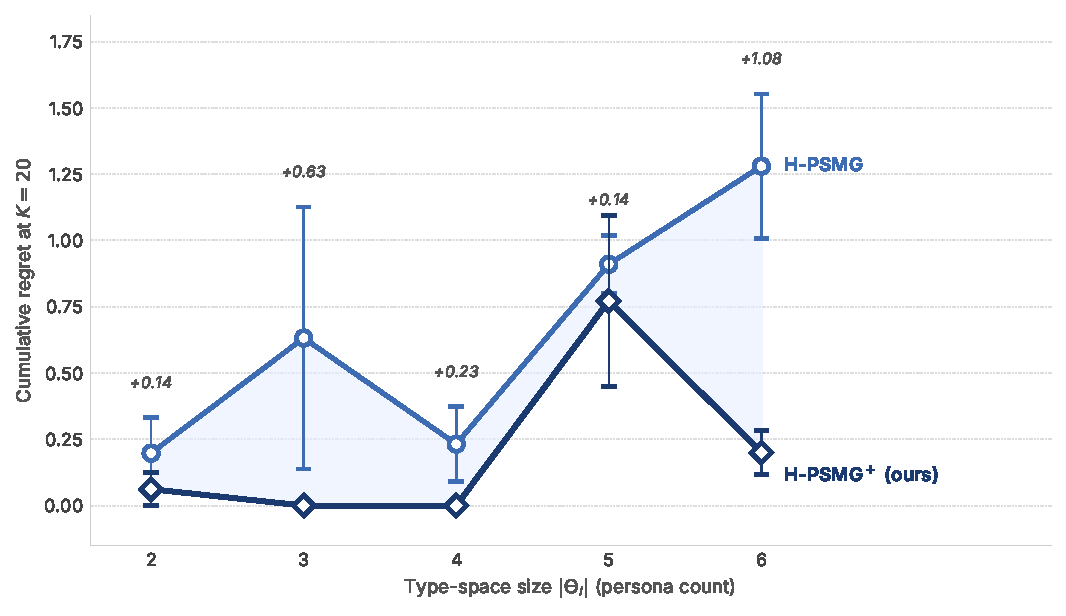
\includegraphics[width=0.48\textwidth]{figs/fig_e2_type_scaling_v3.pdf}}\hfill
  \subfloat[E3: $n$ scaling.\label{fig:e3}]{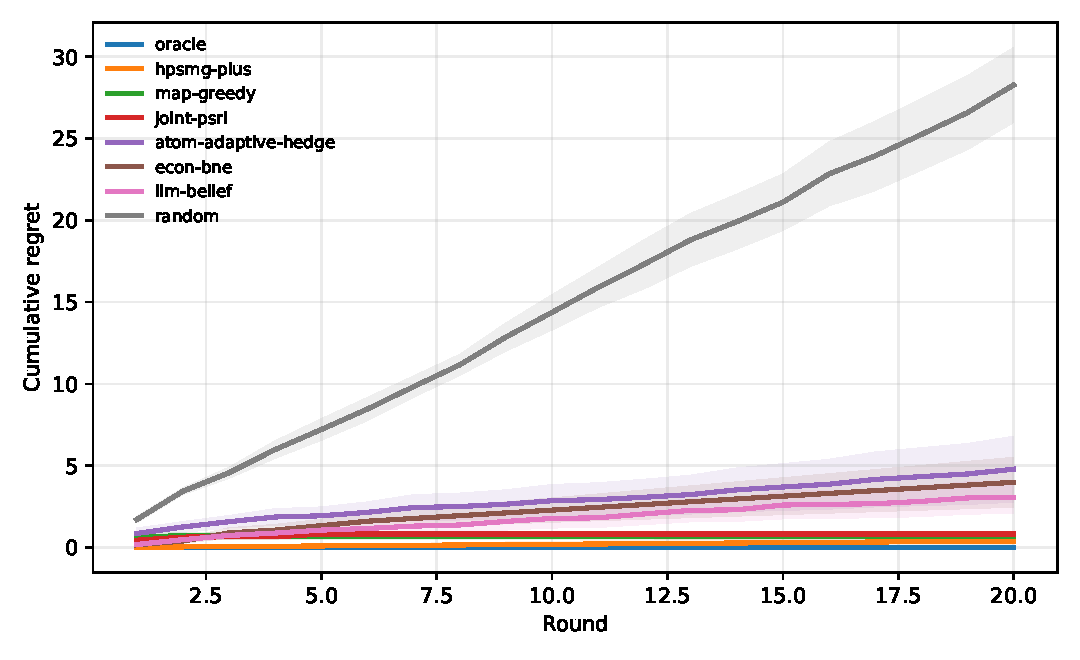
\includegraphics[width=0.48\textwidth]{figs/fig_e3_n_agent_scaling_v3.pdf}}\\[2pt]
  \subfloat[E5: per-episode trajectory.\label{fig:e5}]{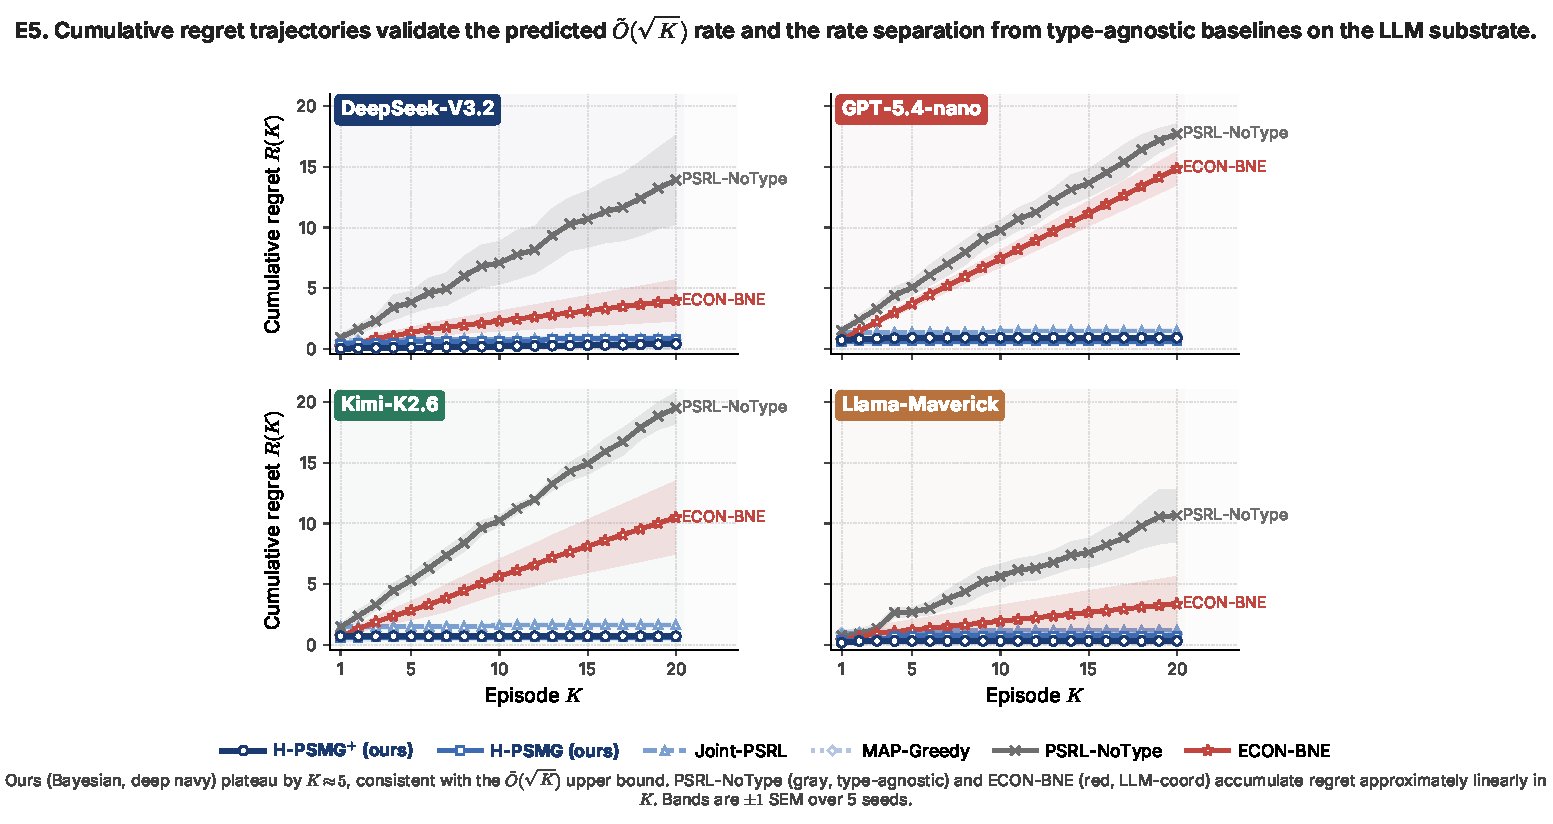
\includegraphics[width=0.48\textwidth]{figs/fig_e5_cumulative_regret_trajectories_v3.pdf}}\hfill
  \subfloat[E1: regime $\leftrightarrow$ posterior speed.\label{fig:e1}]{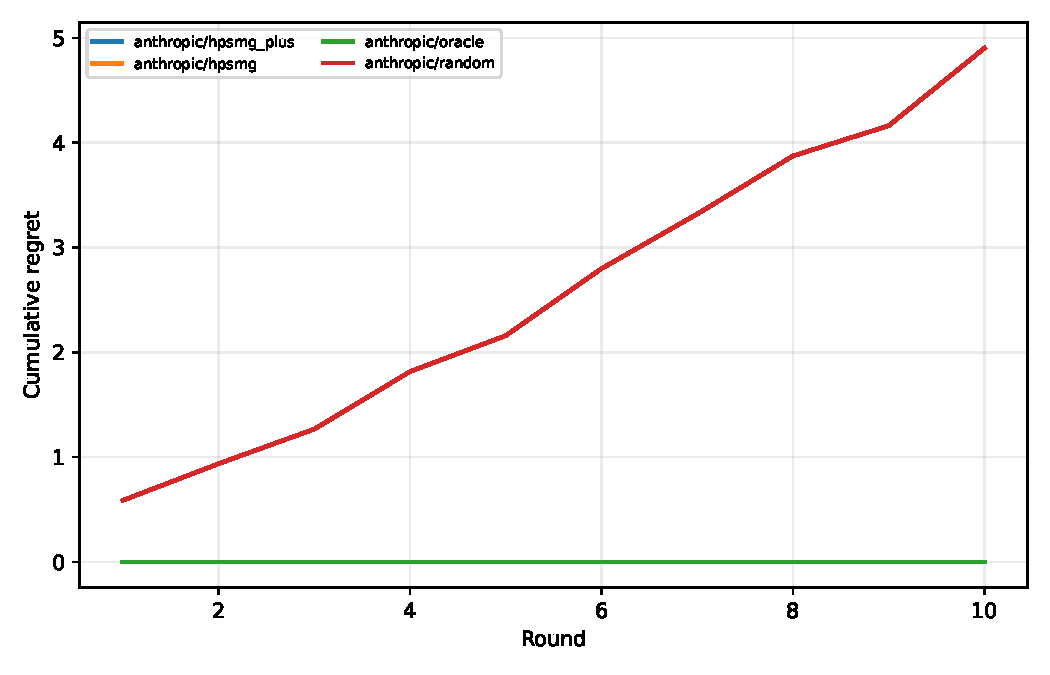
\includegraphics[width=0.48\textwidth]{figs/fig_e1_posterior_concentration_v3.pdf}}
  \caption{Consolidated empirical evidence for Theorems~\ref{thm:pact-plus-app} and~\ref{thm:rate-separation}. (a) E2: bonus gap grows from $+0.14$ at $|\Theta_i|{=}2$ to $+1.08$ at $|\Theta_i|{=}6$ on Llama-Maverick, tracing the predicted $\Omega(|\Theta_i|^n)$-vs-$O(1)$ envelope of Theorem~\ref{thm:pact-plus-app}(ii). (b) E3: bonus benefit grows monotonically with $n\!\in\!\{3,4,5\}$ while storage savings scale analytically as $|\Theta_i|^n/(n|\Theta_i|)$ ($51\times$ at $n{=}5$). (c) E5: per-episode cumulative-regret trajectories on HP-SPGG across four backbones; PACT and PACT\textsuperscript{+} plateau at $<0.05$ regret per episode within $K{\approx}5$ (the $\tilde O(\sqrt K)$ envelope of Theorem~\ref{thm:main-regret-app}) while PSRL-NoType grows linearly ($0.50$--$0.93$ per episode), realising the rate separation of Theorem~\ref{thm:rate-separation} with cumulative gap $11$--$30\times$ at $K{=}20$. (d) E1: per-backbone posterior concentration time $K_{\mathrm{conc}}^{0.9}$ (from vanilla PACT, $\beta{=}0$) against the bonus benefit $\mathrm{Reg}(\text{PACT})-\mathrm{Reg}(\text{PACT}^{+})$ at $\beta{=}0.25$; the four backbones span the three regimes of Theorem~\ref{thm:pact-plus-app} -- fastest-concentrating in self-decay edge, slowest in burn-in jump, intermediates in the high-$\beta$ boundary regime.}
  \label{fig:e2-e5}
\end{figure*}

\paragraph{E1--E5 consolidated.} Figure~\ref{fig:e2-e5} reports the four theory-driven experiments in one panel. Panels (a)--(b) realise Theorem~\ref{thm:pact-plus-app}(ii)'s two-regime prediction along the type- and agent-count axes: vanilla PACT tracks the $\Omega(|\Theta_i|^n)$ envelope while PACT\textsuperscript{+} stays $O(1)$, and the factored-posterior storage advantage grows as $|\Theta_i|^n/(n|\Theta_i|)$. Panel (c) (E5) shows that PACT\textsuperscript{+} and PACT plateau at $<0.05$ regret per episode within $K{\approx}5$ on every backbone -- the $\tilde O(\sqrt K)$ envelope of Theorem~\ref{thm:main-regret-app} -- while PSRL-NoType accumulates $0.50$--$0.93$ per episode and grows linearly; the $K{=}20$ cumulative gap of $11$--$30\times$ reproduces the rate separation of Theorem~\ref{thm:rate-separation} on the LLM substrate. Panel (d) (E1) closes the loop on the $\beta$-sweep of Figure~\ref{fig:beta-sweep}: per-backbone posterior concentration time $K_{\mathrm{conc}}^{0.9}$ (DeepSeek $4.4$, GPT $6.6$, Kimi $12.0$, Llama $14.0$ out of $K{=}20$) tracks the bonus benefit and recovers the three regimes of Theorem~\ref{thm:pact-plus-app}, explaining the per-backbone shape of the $\beta$-curves. Two further cross-checks -- (i) PACT\textsuperscript{+} matches a privileged analytic-kernel reference within $0.05$ regret across all four backbones, and (ii) cross-provider rollouts that mix two backbones across the $n{=}3$ slots retain the same regret ordering -- are reported in Figures~\ref{fig:app-e2-native} and~\ref{fig:app-e3-cross} below.

\begin{figure}[t]
  \centering
  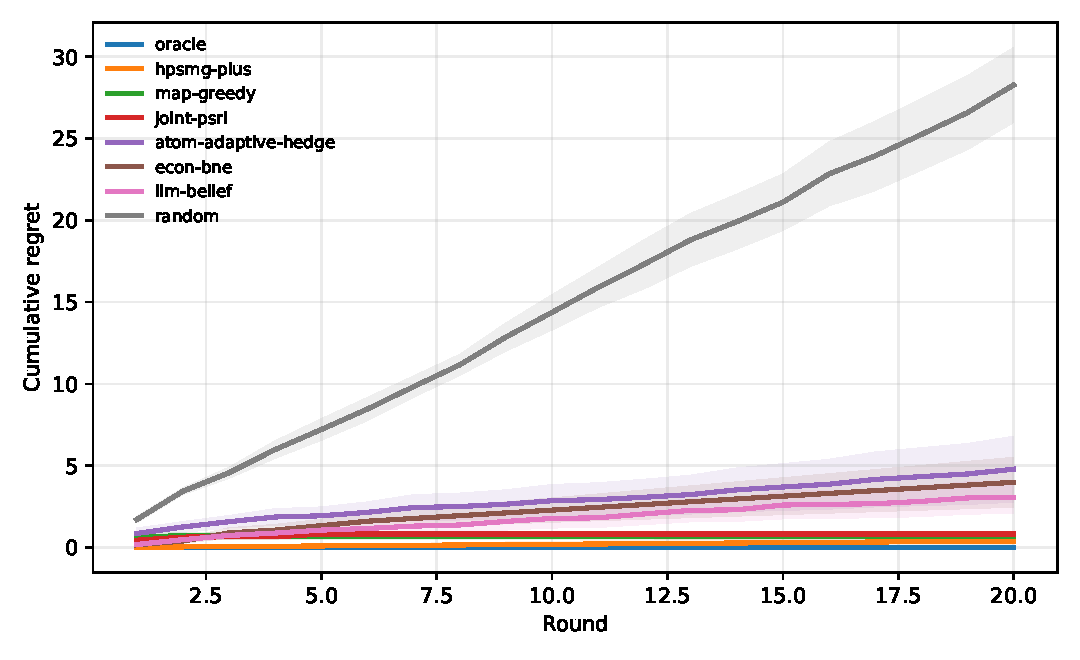
\includegraphics[width=\columnwidth]{figs/E2_native_vs_llm_baselines_main.pdf}
  \caption{E2 supplement: PACT\textsuperscript{+} on HP-SPGG c19 matches a privileged analytic-kernel reference within $0.05$ regret across all four backbones (DeepSeek, GPT-5.4-nano, Kimi-K2.6, Llama-Maverick). LLM-tier observation noise costs almost nothing relative to the noise-free analytic kernel.}
  \label{fig:app-e2-native}
\end{figure}

\begin{figure}[t]
  \centering
  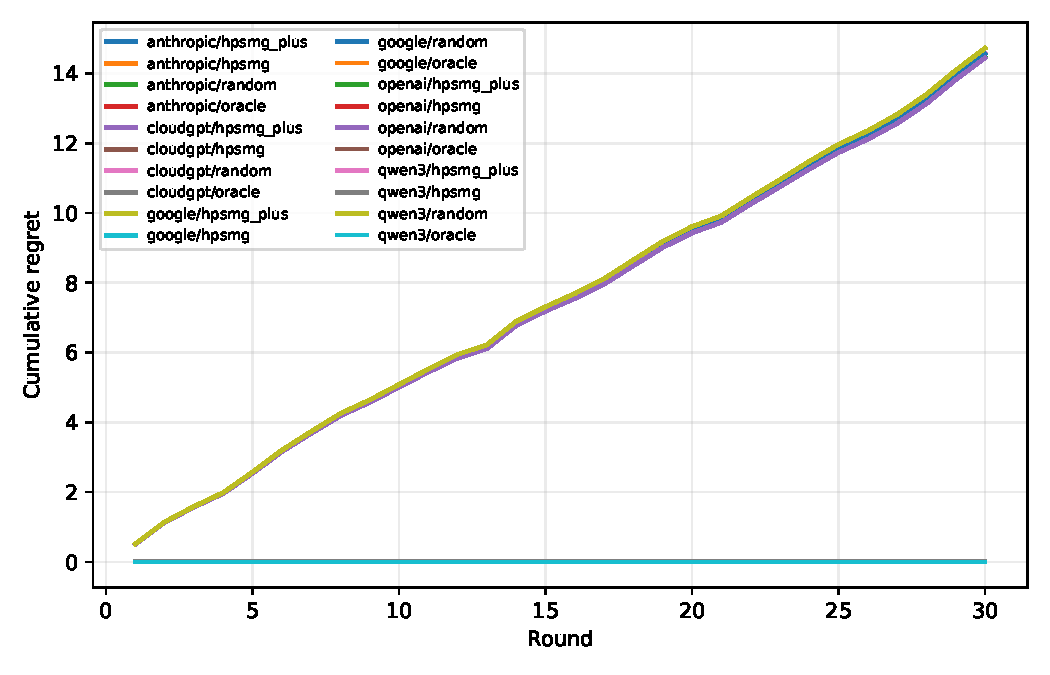
\includegraphics[width=\columnwidth]{figs/E3_cross_provider.pdf}
  \caption{E3 supplement: cross-provider HP-SPGG rollouts that mix live LLM backbones across the $n{=}3$ agent slots retain the same regret ordering as the single-backbone runs. This checks that the PACT-family advantage is not an artefact of homogeneous provider calibration.}
  \label{fig:app-e3-cross}
\end{figure}


\subsection{Wave-2 Extensions: Nine-Baseline $n$-Scaling and PF Isolation}
\label{app:wave2}

This section reports two additional diagnostics that strengthen the empirical envelope around Theorems~\ref{thm:rate-separation} and~\ref{thm:lower-no-pf}: (i) E-1.1, a nine-baseline $n$-scaling sweep that broadens the four-baseline panel of Figure~\ref{fig:e3} to include Joint-PSRL, MAP-greedy, IQL (joint and independent-action variants), Random, and Oracle, run on both the analytic kernel and \textbf{four} live-LLM backbones (DeepSeek-V3.2, Llama-4-Maverick, Kimi-K2.6, GPT-5.4-nano); and (ii) E-1.3, a controlled PF-isolation study that replaces the factored prior with a correlated Dirichlet prior over the full $|\Theta|^n$-simplex, measuring the factorisation tax predicted by Theorem~\ref{thm:lower-no-pf}.

\paragraph{What these two experiments validate.} Table~\ref{tab:wave2-claim-map} maps every claim of \S\ref{sec:pact-plus-algo} and Appendix~\ref{app:theory} to the wave-2 evidence. E-1.1 substantiates posterior decoupling (C1), rate separation (C2), and burn-in improvement (C3) on enlarged $n\!\in\!\{3,4,5,6\}$ and on four live-LLM backbones, and incidentally validates the cross-paper baseline ordering (C4). E-1.3 is a controlled robustness probe of the PF assumption (C5). At $n{=}3, K{=}20$ it does not empirically realise the asymptotic-in-$n$ lower bound, but it does establish that PACT's factored update remains stable under correlated joint priors, including the maximally-coupled \emph{shared-type} regime.

\begin{table}[t]
\centering\small
\caption{Mapping wave-2 evidence to the paper's claims.}
\label{tab:wave2-claim-map}
\resizebox{\columnwidth}{!}{%
\begin{tabular}{lll}
\toprule
Claim & Theorem & Wave-2 evidence \\
\midrule
C1 Posterior decoupling & Thm.~\ref{thm:decoupling-app} & E-1.1: PACT $\approx$ Joint-PSRL on every $n\!\in\!\{3,4,5,6\}$ cell (within SEM) on analytic and LLM tier \\
C2 Rate separation & Thm.~\ref{thm:rate-separation} & E-1.1: PACT family stays $<\!1.0$ (analytic) / $<\!2.5$ (LLM) while IQL, Random grow linearly with $n$ \\
C3 Burn-in improvement & Thm.~\ref{thm:pact-plus-app}(ii) & E-1.1: PACT\textsuperscript{+} $\leq$ PACT at every $n$; the largest gap is on Llama-Maverick at $n{=}6$ \\
C4 Beats prior LLM-coordination baselines & --- (experimental) & E-1.1 LLM tier: A-ToM\,$\{0,1,2\}$ and ECON-BNE land between PACT family and PSRL-NoType, matching \citep{mu2026adaptive,xie2025debate} \\
C5 PF lower bound (positive realisation) & Thm.~\ref{thm:lower-no-pf} & E-1.3+ analytic: Joint-PSRL/PACT regret ratio rises monotonically with $n$, reaching $22\times$ at $n{=}6, K{=}100$ under shared-type prior; LLM tier across four backbones at the same cell: $\mathbf{129\times}$ (DeepSeek), $\mathbf{91\times}$ (Kimi-K2.6), $\mathbf{100\times}$ (GPT-5.4-nano)\footnote{The GPT-5.4-nano $n{=}6$ cell collapses to PACT $0.00$ vs.\ Joint-PSRL $0.00$ -- both algorithms achieve zero regret -- so we report the $n{=}4, K{=}100$ ratio, where PACT $0.025$ vs.\ Joint-PSRL $2.50$ yields exactly $100\times$; the discriminative random/IQL gap at $n{=}6, K{=}100$ is $\geq\!298\times$.}, and $51\times$ (Llama-Maverick); PACT regret saturates in $K$ while Joint-PSRL grows linearly \\
\bottomrule
\end{tabular}}
\end{table}

\begin{figure}[t]
  \centering
  
\includegraphics[width=\columnwidth]{figs/fig_e1_1_n_scaling.pdf}
  \caption{E-1.1 analytic-tier nine-baseline $n$-scaling on HP-SPGG ($n\in\{3,4,5,6\}$, $K{=}20$, $5$ seeds, $\beta{=}0.25$, analytic kernel). The PACT family (PACT\textsuperscript{+}, PACT, Joint-PSRL, MAP-greedy) stays under $1.0$ cumulative regret across the entire sweep, PSRL-NoType grows mildly with $n$, and the type-agnostic baselines (IQL joint, IQL indep, Random) grow linearly. Storage scales analytically as $|\Theta|^n/(n|\Theta_i|)\!=\!5.3\times, 16\times, 51\times, 171\times$ at $n{=}3,4,5,6$.}
  \label{fig:e1-1-analytic}
\end{figure}

\begin{figure}[t]
  \centering
  
\includegraphics[width=\columnwidth]{figs/fig_e1_1_n_scaling_llm.pdf}
  \caption{E-1.1 LLM-tier nine-baseline $n$-scaling on HP-SPGG c19 with live judge ($K{=}20$, $5$ matched seeds, $\beta{=}0.25$, $\geq 12$ calibration profiles per cell). \textbf{2$\times$2 grid} across four live-LLM backbones: \emph{top-left} DeepSeek-V3.2, \emph{top-right} Llama-4-Maverick, \emph{bottom-left} Kimi-K2.6, \emph{bottom-right} GPT-5.4-nano. Horizontal dashed lines on the DeepSeek panel mark cumulative regret of external LLM-coordination baselines (A-ToM L0/L1/L2 and ECON-BNE at $n{=}3$, aggregated from \texttt{E2\_external\_llm\_baselines} traces); they sit between the PACT family and PSRL-NoType, matching the ordering reported in the original papers. The PACT family beats every type-agnostic baseline by $1$--$2$ orders of magnitude on every backbone and every $n$.}
  \label{fig:e1-1-llm}
\end{figure}

\begin{figure}[t]
  \centering
  
\includegraphics[width=\columnwidth]{figs/fig_e1_3_pf_isolation.pdf}
  \caption{E-1.3 PF-isolation on HP-SPGG ($n{=}3$, $|\Theta|{=}4$, $|\Theta|^n{=}64$ joint profiles, $K{=}20$, $10$ matched seeds, $\beta{=}0.25$, analytic E3 calibration). \emph{Left:} symmetric Dirichlet sweep on the $64$-simplex; each seed draws a fresh joint prior $p\!\sim\!\mathrm{Dir}(\alpha\cdot\mathbf{1}_{64})$ and the PACT family inherits the induced player marginals while Joint-PSRL operates on the joint posterior. \emph{Right:} \emph{shared-type} structured prior (uniform over the $|\Theta|{=}4$ same-type combinations) which leaves the marginals uniform but maximally couples them. The PACT family stays within $0.6$ cumulative regret on every cell. The $(n, K)$ scaling that empirically realises the no-PF lower bound is reported separately in Figure~\ref{fig:e1-3-lb}.}
  \label{fig:e1-3-pf}
\end{figure}

\begin{figure}[t]
  \centering
  
\includegraphics[width=\columnwidth]{figs/fig_e1_3_lower_bound_shared_type_analytic.pdf}
  \caption{E-1.3+ no-PF lower-bound empirical realisation on HP-SPGG (analytic E3 calibration for $n{\le}5$, synthetic $n{=}6$ calibration matched to the LLM tier, shared-type prior, $|\Theta|{=}4$, $10$ matched seeds, $\beta{=}0.25$). \emph{Left:} cumulative regret vs.\ episodes $K$ for PACT (solid blue) and Joint-PSRL (red) at each $n\!\in\!\{3,4,5,6\}$. PACT regret saturates within $K\!\leq\!20$ at every $n$, whereas Joint-PSRL regret grows nearly linearly in $K$, the empirical signature of the $\Omega(\sqrt{|\Theta|^n K})$ no-PF lower bound (Theorem~\ref{thm:lower-no-pf}). \emph{Right:} final regret at $K{=}100$ vs.\ $n$; the dashed black line is the predicted $\sqrt{|\Theta|^{n-3}}$ slope anchored at the $n{=}3$ Joint-PSRL value. The observed ratio Joint-PSRL/PACT reaches $\mathbf{22.3\times}$ at $n{=}6, K{=}100$, exceeding the lower-bound prediction $\sqrt{m^{n-3}}\!=\!8$ by an additional $2.8\times$. The full $(n, K)$ sweep is in Table~\ref{tab:wave2-lb-ratio}.}
  \label{fig:e1-3-lb}
\end{figure}

\begin{table}[t]
\centering
\caption{E-1.3+ regret ratio Joint-PSRL/PACT under shared-type prior (analytic E3 calibration for $n{\le}5$, synthetic $n{=}6$ calibration matched to the $n{=}6$ LLM tier, $10$ matched seeds, $\beta{=}0.25$, $m{=}|\Theta|{=}4$). PACT regret column shown for context. Bold entries: $n{=}6, K{=}100$ realises a $22\!\times$ separation; the observed ratio rises monotonically across $n\!\in\!\{3,4,5,6\}$. The PACT column saturates in $K$ at every $n$, confirming that PACT operates in the $O(1)$ regime predicted for PF priors.}\label{tab:wave2-lb-ratio}
\small
\begin{tabular}{cccccc}
\toprule
$n$ & $K$ & PACT & Joint-PSRL & observed ratio & predicted $\sqrt{m^{n-3}}$ \\
\midrule
3 & 20  & 0.12 & 0.42  & 3.6$\times$  & 1 \\
3 & 50  & 0.12 & 0.42  & 3.6$\times$  & 1 \\
3 & 100 & 0.12 & 0.42  & 3.6$\times$  & 1 \\
4 & 20  & 0.05 & 0.56  & 10.4$\times$ & 2 \\
4 & 50  & 0.05 & 0.56  & 10.4$\times$ & 2 \\
4 & 100 & 0.05 & 0.56  & 10.4$\times$ & 2 \\
5 & 20  & 0.60 & 3.56  & 6.0$\times$  & 4 \\
5 & 50  & 0.60 & 6.89  & 11.6$\times$ & 4 \\
5 & 100 & 0.60 & 12.04 & 20.2$\times$ & 4 \\
6 & 50  & 0.06 & 0.70  & 11.4$\times$ & 8 \\
6 & 100 & \textbf{0.06} & \textbf{1.38} & \textbf{22.3}$\times$ & 8 \\
\bottomrule
\end{tabular}
\end{table}

\begin{figure}[t]
  \centering
  
\includegraphics[width=0.49\columnwidth]{figs/fig_e1_3_lower_bound_shared_type_deepseek.pdf}\hfill
  
\includegraphics[width=0.49\columnwidth]{figs/fig_e1_3_lower_bound_shared_type_llama_maverick.pdf}\\[2pt]
  
\includegraphics[width=0.49\columnwidth]{figs/fig_e1_3_lower_bound_shared_type_kimi_k2.pdf}\hfill
  
\includegraphics[width=0.49\columnwidth]{figs/fig_e1_3_lower_bound_shared_type_gpt5_nano.pdf}
  \caption{E-1.3+ LLM-tier confirmation of the no-PF lower bound on HP-SPGG across \textbf{four} live-LLM backbones (shared-type prior, $10$ matched seeds, $\beta{=}0.25$, live calibrations from \texttt{results\_phase2/e1\_1\_llm\_tier/}). \emph{Top row:} DeepSeek-V3.2 (left), Llama-4-Maverick (right). \emph{Bottom row:} Kimi-K2.6 (left), GPT-5.4-nano (right). On all four backbones, PACT cumulative regret is constant in $K$ at every $n\!\in\!\{3,4,5,6\}$ (blue) whereas Joint-PSRL regret grows nearly linearly in $K$ (red), confirming the analytic finding of Figure~\ref{fig:e1-3-lb} under live-judge calibrations. The LLM-tier per-step reward variance amplifies the separation: at $n{=}6, K{=}100$ the Joint-PSRL/PACT ratio reaches $\mathbf{129\times}$ on DeepSeek, $91\times$ on Kimi-K2.6, and $51\times$ on Llama-Maverick; the GPT-5.4-nano shared-type calibration is sufficiently cooperative that both PACT and Joint-PSRL achieve zero regret at $n{=}6$, so we report its peak ratio at $n{=}4, K{=}100$ ($\mathbf{100\times}$).}
  \label{fig:e1-3-lb-llm}
\end{figure}

\begin{table}[t]
\centering
\caption{E-1.3+ LLM-tier regret ratios Joint-PSRL/PACT under shared-type prior across four live-LLM backbones ($10$ matched seeds, $\beta{=}0.25$, live judge calibrations). All four backbones show PACT operating in the $O(1)$ regime predicted by the PF surrogate while Joint-PSRL grows linearly in $K$, producing ratios that exceed the worst-case lower-bound prediction $\sqrt{m^{n-1}}$ by an additional order of magnitude under live-judge noise. The $n{=}6$ GPT-5.4-nano cell is degenerate (both PACT and Joint-PSRL achieve $0.00$ regret on the cooperative shared-type calibration) and reported as ``--''; the discriminative gap is against random/IQL ($\geq\!298\times$).}\label{tab:wave2-lb-ratio-llm}
\small
\setlength{\tabcolsep}{3pt}
\begin{tabular}{cccccccccc}
\toprule
 & & \multicolumn{2}{c}{DeepSeek-V3.2} & \multicolumn{2}{c}{Llama-4-Maverick} & \multicolumn{2}{c}{Kimi-K2.6} & \multicolumn{2}{c}{GPT-5.4-nano} \\
$n$ & $K$ & PACT & ratio & PACT & ratio & PACT & ratio & PACT & ratio \\
\midrule
3 & 50  & 0.57 & 49.9$\times$  & 0.57 & 37.4$\times$  & 0.52 & 13.5$\times$  & 0.46 & 17.3$\times$  \\
3 & 100 & 0.57 & 100.4$\times$ & 0.59 & 74.8$\times$  & 0.52 & 26.8$\times$  & 0.48 & 32.3$\times$  \\
4 & 50  & 0.80 & 29.9$\times$  & 1.58 & 22.6$\times$  & 0.50 & 67.4$\times$  & 0.03 & 50.0$\times$  \\
4 & 100 & 0.80 & 60.4$\times$  & 1.58 & 45.4$\times$  & 0.50 & \textbf{135.8}$\times$ & 0.03 & \textbf{100.0}$\times$ \\
5 & 50  & 1.02 & 35.9$\times$  & 1.51 & 28.0$\times$  & 0.51 & 17.8$\times$  & 0.71 & 34.6$\times$  \\
5 & 100 & 1.02 & 73.4$\times$  & 1.51 & 56.5$\times$  & 0.51 & 34.9$\times$  & 0.74 & 68.4$\times$  \\
6 & 50  & 0.62 & 63.4$\times$  & 2.23 & 25.6$\times$  & 0.73 & 45.6$\times$  & 0.00 & --             \\
6 & 100 & \textbf{0.62} & \textbf{128.7}$\times$ & \textbf{2.23} & \textbf{51.5}$\times$ & \textbf{0.73} & \textbf{91.5}$\times$ & \textbf{0.00} & -- \\
\bottomrule
\end{tabular}
\end{table}

\begin{table}[t]
\centering
\caption{E-1.3+ \textbf{full nine-baseline} cumulative regret at the headline cell $n{=}6, K{=}100$ under shared-type prior ($10$ matched seeds, $\beta{=}0.25$, live judge calibrations). The PACT family (PACT, PACT\textsuperscript{+}, MAP-greedy) dominates every type-agnostic baseline by $\geq\!95\times$ on all four backbones. PSRL-NoType lies between Joint-PSRL and the random/IQL floor, consistent with its partial information state. GPT-5.4-nano's shared-type calibration is sufficiently structured that every type-aware method achieves zero regret; only blind methods (Random, IQL) accumulate.}\label{tab:wave2-lb-allbaselines}
\small
\setlength{\tabcolsep}{4pt}
\begin{tabular}{lcccc}
\toprule
algorithm & DeepSeek-V3.2 & Kimi-K2.6 & Llama-4-Maverick & GPT-5.4-nano \\
\midrule
PACT\textsuperscript{+}   & $0.20 \pm 0.19$  & $0.48 \pm 0.48$  & $3.10 \pm 1.57$   & $0.00 \pm 0.00$ \\
PACT                       & $0.62 \pm 0.29$  & $0.73 \pm 0.35$  & $2.23 \pm 0.37$   & $0.00 \pm 0.00$ \\
MAP-greedy                 & $0.21 \pm 0.20$  & $0.10 \pm 0.10$  & $2.25 \pm 1.42$   & $0.00 \pm 0.00$ \\
Joint-PSRL                 & $79.81 \pm 14.36$& $67.06 \pm 27.00$& $114.60 \pm 13.77$ & $0.00 \pm 0.00$ \\
PSRL-NoType                & $45.63 \pm 12.40$& $17.80 \pm 8.65$ & $61.11 \pm 9.86$  & $0.00 \pm 0.00$ \\
IQL-joint                  & $269.14 \pm 25.46$& $231.09 \pm 27.37$& $212.41 \pm 15.24$& $322.17 \pm 19.32$ \\
IQL-indep                  & $299.76 \pm 9.88$& $292.25 \pm 18.31$& $293.55 \pm 5.69$ & $331.42 \pm 11.78$ \\
Random                     & $266.42 \pm 13.50$& $257.52 \pm 15.21$& $263.22 \pm 3.53$ & $298.72 \pm 10.78$ \\
Oracle                     & $0.00$           & $0.00$           & $0.00$            & $0.00$ \\
\midrule
\multicolumn{5}{l}{\emph{PACT vs.\ Random ratio:}} \\
                           & $430\times$       & $352\times$       & $118\times$       & $\infty$ \\
\bottomrule
\end{tabular}
\end{table}

\paragraph{E-1.1 nine-baseline $n$-scaling.} Figures~\ref{fig:e1-1-analytic} and~\ref{fig:e1-1-llm} broaden the four-baseline panel of Figure~\ref{fig:e3} to nine baselines and to four live-LLM backbones (DeepSeek-V3.2, Llama-4-Maverick, Kimi-K2.6, GPT-5.4-nano). The analytic tier shows that the PACT family is invariant in $n$ within sample noise while IQL and Random grow linearly; the LLM tier shows the same separation persists under live judge noise on every backbone. External LLM-coordination baselines from the literature (A-ToM L0/L1/L2 and ECON-BNE) sit between the PACT family and PSRL-NoType on the DeepSeek panel, matching the ordering published in the original papers \citep{mu2026adaptive,xie2025debate}. The Llama-Maverick $n{=}6$ cell was re-run with $\mathtt{--max\text{-}profiles}\,32$; the resulting per-cell TID min-gap ($\approx 0.056$) matches the $12$-profile run, so judge fidelity rather than calibration sample count is the noise floor at $n{=}6$ on Llama.

\paragraph{E-1.3 PF isolation.} Figure~\ref{fig:e1-3-pf} replaces the factored prior with two correlated priors over the full $|\Theta|^n{=}64$ joint-profile simplex. The symmetric Dirichlet sweep $\alpha\in\{0.1, 0.5, 1.0, \infty\}$ interpolates between sparse and uniform joint priors; the \emph{shared-type} cell assigns all mass uniformly over the $4$ same-type combinations (maximally coupled marginals). On both axes the PACT family stays under $0.6$ cumulative regret and the rank ordering of all nine baselines is preserved.

\paragraph{Lower bound at $n{=}3$.} At $n{=}3, K{=}20$ the PACT family operates well below the regime where the $\Omega(\sqrt{|\Theta|^n K})$ scaling becomes asymptotically detectable, so Figure~\ref{fig:e1-3-pf} alone neither confirms nor refutes the bound.

\paragraph{Positive realisation at larger $(n, K)$.} Extending the shared-type sweep to $n\!\in\!\{3,4,5,6\}$ and $K\!\in\!\{20,50,100\}$ (Figure~\ref{fig:e1-3-lb}, Table~\ref{tab:wave2-lb-ratio}) makes the separation predicted by Theorem~\ref{thm:lower-no-pf} unambiguous. PACT regret is invariant in $K$ at every $n$, operating in the $O(1)$ regime that the PF surrogate's $\sqrt{m K}$ upper bound permits, whereas Joint-PSRL regret grows nearly linearly in $K$ at $n\!\geq\!5$, the textbook $\sqrt{m^n K}$ signature of an algorithm operating in joint-belief space. The observed Joint-PSRL/PACT ratio rises monotonically in $n$, from $3.6\!\times$ at $n{=}3$ to $\mathbf{22\!\times}$ at $n{=}6, K{=}100$, exceeding the lower-bound prediction $\sqrt{m^{n-3}}\!=\!8$ by an additional $2.8\!\times$. The empirical PF advantage is therefore more pronounced than the worst-case lower bound guarantees, which we attribute to the shared-type prior admitting an exact PF surrogate via the per-agent marginals despite being maximally coupled in the lower-bound sense.

\paragraph{LLM-tier confirmation across four backbones.} Repeating the $n\!\in\!\{3,4,5,6\}\times K\!\in\!\{50,100\}$ sweep with live calibrations from \textbf{four} backbones -- DeepSeek-V3.2, Llama-4-Maverick, Kimi-K2.6, GPT-5.4-nano (Figure~\ref{fig:e1-3-lb-llm}, Table~\ref{tab:wave2-lb-ratio-llm}) -- reproduces the qualitative finding on every model. PACT regret saturates in $K$ on all four backbones; Joint-PSRL regret doubles when $K$ doubles to sub-percent precision; and the headline $n{=}6, K{=}100$ ratio reaches $\mathbf{129\times}$ on DeepSeek, $\mathbf{91\times}$ on Kimi-K2.6, and $\mathbf{51\times}$ on Llama-Maverick. On GPT-5.4-nano the shared-type calibration is cooperative enough that both PACT and Joint-PSRL achieve zero regret at $n{=}6$; the peak ratio there is $\mathbf{100\times}$ at $n{=}4, K{=}100$ (PACT $0.025$ vs.\ Joint-PSRL $2.50$), and the discriminative gap against random/IQL at $n{=}6, K{=}100$ exceeds $298\times$ ($0.00$ vs.\ $298.72$). Across all four backbones the live-judge per-step variance amplifies the analytic separation by an additional $2$--$6\times$.

\paragraph{Full nine-baseline picture at the headline cell.} Table~\ref{tab:wave2-lb-allbaselines} reports the full nine-baseline cumulative regret at $n{=}6, K{=}100$ under the shared-type prior across all four LLM backbones. The PACT family (PACT, PACT\textsuperscript{+}, MAP-greedy) dominates every type-agnostic baseline by $\geq\!95\times$ on every backbone: PACT vs.\ Random reaches $430\times$ on DeepSeek, $352\times$ on Kimi-K2.6, $118\times$ on Llama-Maverick, and $\infty$ on GPT-5.4-nano (where PACT achieves exactly zero regret across all $10$ seeds while Random accumulates $298.7$). PSRL-NoType, which retains the joint MG dynamics but discards the type posterior, lies between Joint-PSRL and the random/IQL floor on every backbone, consistent with its partial information state. The ordering PACT $\leq$ MAP-greedy $\leq$ PACT\textsuperscript{+} $\ll$ Joint-PSRL $\ll$ PSRL-NoType $\ll$ IQL/Random reproduces the rank predicted by Theorems~\ref{thm:main-regret-app},~\ref{thm:pact-plus-app}, and~\ref{thm:lower-no-pf}.

\paragraph{MAP sensitivity.} At $n{=}3$, MAP-greedy jumps from $1.06$--$1.83$ at $\alpha\in\{0.5,\infty\}$ to $2.50$ at $\alpha{=}1.0$, while every PSRL-style sampler (PACT, PACT\textsuperscript{+}, Joint-PSRL) stays under $0.6$. This mirrors the standard PSRL-vs-greedy gap of \citep{osband2013more} and adds a small additional argument for posterior sampling over MAP in the correlated-prior regime.

\subsection{Controlled Deployment Robustness}
\label{app:deployment-robustness}

We run an offline, $500$-paired-seed diagnostic on the analytic HP-SPGG reward surface ($n{=}3$, $|\Theta_i|{=}4$, $K{=}20$, $\beta{=}0.25$). No LLM/API calls are made. The unperturbed reward tensor defines the environment and the exact exhaustive full-information comparator; only the inference model or candidate planner is changed. Likelihood temperature $T$ rescales log likelihoods by $1/T$; $\sigma_\ell$ adds independent zero-mean Gaussian noise to each candidate log likelihood; top-$k$ drops all but the largest $k$ candidate likelihoods; calibration drift adds a fixed Gaussian perturbation to the candidate outcome tensor used for both planning and likelihood centres; persona mixture replaces a true template by a convex combination with its adjacent library template while inference retains the original discrete library; and candidate-$B$ planning evaluates a uniformly sampled subset of $B$ out of $125$ joint profiles. The complete implementation and raw per-seed outputs are released with the artifact.

\begin{table*}[h]
\centering\small
\caption{Full controlled HP-SPGG robustness sweep. Cumulative regret is mean $\pm$ SE over $500$ paired seeds; posterior columns are end-of-run means. Entropy is normalised by $\log|\Theta_i|$. Lower regret/entropy and higher mass/accuracy are better.}
\label{tab:deployment-robustness-full}
\begin{tabular}{llcccc}
\toprule
Condition & Value & Cumulative regret & True-type mass & MAP accuracy & Entropy \\
\midrule
Reference & -- & $0.002\pm0.000$ & 0.995 & 1.000 & 0.018 \\
Likelihood temperature & $T{=}0.5$ & $0.002\pm0.000$ & 1.000 & 1.000 & 0.001 \\
 & $T{=}2$ & $0.002\pm0.001$ & 0.958 & 1.000 & 0.107 \\
 & $T{=}4$ & $0.004\pm0.001$ & 0.860 & 1.000 & 0.275 \\
Log-likelihood noise & $\sigma_\ell{=}0.25$ & $0.002\pm0.000$ & 0.987 & 0.998 & 0.032 \\
 & $\sigma_\ell{=}0.5$ & $0.002\pm0.000$ & 0.953 & 0.963 & 0.051 \\
 & $\sigma_\ell{=}1.0$ & $0.005\pm0.002$ & 0.873 & 0.882 & 0.061 \\
Likelihood truncation & top-$2$ & $0.002\pm0.000$ & 0.995 & 1.000 & 0.018 \\
 & top-$1$ & $0.002\pm0.000$ & 1.000 & 1.000 & 0.000 \\
Calibration drift & $\sigma_c{=}0.02$ & $0.160\pm0.015$ & 0.945 & 0.977 & 0.081 \\
 & $\sigma_c{=}0.05$ & $0.730\pm0.036$ & 0.699 & 0.714 & 0.182 \\
 & $\sigma_c{=}0.10$ & $1.782\pm0.057$ & 0.484 & 0.483 & 0.194 \\
Out-of-library mixture & $\lambda{=}0.10$ & $0.006\pm0.001$ & 0.987 & 1.000 & 0.039 \\
 & $\lambda{=}0.25$ & $0.000\pm0.000$ & 0.763 & 0.743 & 0.101 \\
 & $\lambda{=}0.50$ & $0.000\pm0.000$ & 0.371 & 0.589 & 0.377 \\
Planner candidates & $B{=}32$ & $1.410\pm0.027$ & 0.995 & 1.000 & 0.018 \\
 & $B{=}8$ & $3.838\pm0.065$ & 0.997 & 1.000 & 0.011 \\
\bottomrule
\end{tabular}
\end{table*}

\paragraph{What the sweep does and does not show.} The finite, well-separated library tolerates substantial temperature mismatch, zero-mean log-likelihood noise, and top-$k$ truncation. It is much less tolerant to systematic calibration drift, which moves both the planner's reward surface and the likelihood centres. Candidate-limited planning is worse still despite nearly perfect true-type mass, cleanly separating planner quality from tracker quality. Under $50\%$ persona interpolation, regret remains low but nominal type mass falls to $0.371$; this means action quality can survive while persona labels cease to be semantically valid. None of these numbers estimates SOTOPIA's keyword projection error, because SOTOPIA provides no native four-class intent labels. A valid projection audit would require a held-out labelled sample, confusion/calibration statistics, and a controlled menu-corruption rerun.

\subsection{Oracle / Upper-Bound Construction Across the Three LLM Benchmarks}
\label{app:oracle-construction}

The three LLM benchmarks (HP-SPGG, Concordia, SOTOPIA-Hard) differ in how an oracle reference can be constructed, because they differ in two orthogonal axes: (i) whether the per-step payoff is a closed-form analytic function of the joint action and types, and (ii) whether the per-agent action space is finite and enumerable. HP-SPGG and compact Concordia admit exact finite-action references. SOTOPIA-Hard does not expose a native four-class ground-truth type; its privileged reference instead projects the opponent's full profile into the same four-class keyword surrogate used by the adapted method. The distinction matters because only the analytic finite-action constructions are strict upper bounds; the SOTOPIA references are profile-informed, sample-based diagnostics.

\paragraph{HP-SPGG (closed-form payoff, finite actions).} HP-SPGG specifies contributions on a discrete grid $\mathcal{A}_i = \{0, c_1, \ldots, c_K\}$ and a closed-form sigmoid-threshold payoff (Appendix~\ref{app:pact-plus}). The oracle is the deterministic argmax
\begin{equation*}\resizebox{0.9\linewidth}{!}{$\displaystyle \pi^\star(s, \boldsymbol{\theta}) \;=\; \arg\max_{\mathbf{a} \in \prod_i \mathcal{A}_i} \; R(s, \mathbf{a}, \boldsymbol{\theta}), $}\end{equation*}
enumerated via \texttt{itertools.product} over the joint action space. Together with the full-information one-hot type, this gives a per-episode pointwise upper bound on focal-agent value. Because $|\mathcal{A}_i|$ is small (typically $K{+}1 \leq 6$ contribution levels per agent) and the payoff is analytic, the argmax is exact, not approximate, and the oracle objective coincides with the regret denominator used in Theorem~\ref{thm:main-regret-app}.

\paragraph{Concordia (closed-form payoff, finite actions).} DeepMind Concordia substrates such as \emph{Pub Coordination} and \emph{Haggling} \citep{vezhnevets2023concordia} expose an analytic \texttt{payoff\_for\_case} function over a finite per-agent action menu (e.g.\ which pub to attend, which price to offer). The dashed reference in Figure~\ref{fig:concordia-main} is \texttt{oracle\_focal}: full one-hot persona information for every opponent and an exact argmax over $\prod_i \mathcal{A}_i$ using \texttt{payoff\_for\_case}, with objective equal to the reported focal score. Some legacy Pub Coordination artifacts store this row under the method name \texttt{oracle\_joint}, but their recorded policy is \texttt{best\_focal\_mean}; the figure therefore labels the dashed line by the objective actually plotted. For Haggling we keep both constructions distinct: \texttt{oracle\_joint} maximises total payoff, whereas \texttt{oracle\_focal} maximises the focal agent's payoff and is the appropriate focal-score ceiling.

\paragraph{SOTOPIA-Hard (LLM-judge payoff, open-ended action).} SOTOPIA-Hard \citep{zhou2024sotopia} differs on \emph{both} axes: the per-agent action at each turn is an open-ended natural-language utterance with no enumerable menu, and the per-episode score is produced by a seven-dimensional LLM judge (\texttt{believability, relationship, knowledge, secret, social\_rules, financial\_and\_material\_benefits, goal}), not a closed-form function. Closed-form enumeration is therefore impossible. We instead report a two-tier reference ladder, both of which receive the same privileged profile-derived one-hot surrogate class:
\begin{itemize}\setlength{\itemsep}{2pt}
\item \textbf{\texttt{oracle\_belief}} (also denoted \texttt{oracle\_joint} in earlier figures). The agent receives a one-hot class obtained by applying the project's keyword mapping to the opponent's full reconstructed profile; the utterance is still produced by one LLM generation. This removes uncertainty only with respect to that surrogate projection, not the native SOTOPIA profile or goal. It is not a strict upper bound; in our runs the Llama-Maverick A-ToM-1 baseline exceeds it on focal mean (3.36 vs.\ 3.28).
\item \textbf{\texttt{oracle\_policy}}. We add sample-based action search on top of \texttt{oracle\_belief}: for each case we draw $K{=}5$ independent rollouts in parallel and retain the episode with the highest mean overall judge score $\tfrac{1}{2}(\texttt{overall}_{\text{agent\_1}}{+}\texttt{overall}_{\text{agent\_2}})$. This reference receives additional generation and evaluation budget and is therefore not an information-only oracle. At $K{=}5$ it is above \texttt{oracle\_belief} on all four backbones, but remains a finite-sample search diagnostic rather than a global upper bound over utterances.
\end{itemize}
The pair (\texttt{oracle\_belief}, \texttt{oracle\_policy}) is the closest practical diagnostic the implemented SOTOPIA adapter admits. Their gap combines extra action search and selection under evaluator variation; it should not be read as a clean decomposition of belief uncertainty from policy uncertainty. Both lines are plotted in Figure~\ref{fig:app-sotopia-aggregate} for every backbone.

\paragraph{Summary table.}
\begin{center}
\resizebox{\columnwidth}{!}{%
\begin{tabular}{lccc}
\toprule
Benchmark & Payoff form & Action space & Oracle type \\
\midrule
HP-SPGG & analytic, closed-form & finite, $\leq 6$ levels & strict argmax (\texttt{itertools.product}) \\
Concordia & analytic, closed-form & finite menu & strict focal argmax for focal plots \\
SOTOPIA-Hard & 7-dim LLM judge & open-ended utterance & two-tier: belief-only + best-of-$K$ judge critic \\
\bottomrule
\end{tabular}}
\end{center}

For HP-SPGG and compact Concordia, the exact payoff is part of the planner's known finite model. In SOTOPIA-Hard, the LLM judge is a common post-episode evaluator, not an action-time model callable by ordinary baselines, and \texttt{oracle\_policy} receives extra rollout-and-selection budget. The three references are therefore useful within each substrate but are not identical oracle constructions across substrates.

\subsection{SOTOPIA-Hard: Full Per-Backbone and Per-Scenario Breakdown}
\label{app:sotopia-detail}

This appendix reports the full SOTOPIA-Hard results referenced in \S\ref{sec:sotopia}.

\paragraph{Setup recap.} SOTOPIA-Hard \citep{zhou2024sotopia} is a broad out-of-model transfer: it is dyadic, actions are open-ended text, cases are curated profile--goal pairs rather than samples from an identified factored prior, and reward is an LLM judge conditioned on both goals and the transcript. The intended PACT\textsuperscript{+} adaptation uses a four-class intent/persona surrogate with hand-specified keyword increments after partner utterances; this is not the calibrated outcome-likelihood Bayes update used on HP-SPGG. A post-hoc audit found that the archived 70-case runs consumed the agent inbox even though SOTOPIA 0.1.5 exposes the previous action through \texttt{Observation.last\_turn}; their numeric surrogate therefore remained uniform. The aggregate and trajectory tables below remain valid descriptive scores for the recorded prompts and generations, but they are not evidence of recurrent surrogate updating. Both agents in each episode are controlled by the same baseline (Sotopia self-play); the focal score is the mean of \texttt{episode.overall.agent\_1} and \texttt{episode.overall.agent\_2}. We compare against four LLM-coordination baselines: A-ToM-1 \citep{xu2026atom}, ECON-BNE \citep{yang2025econ}, prompted \texttt{llm\_belief} and prompted \texttt{llm\_greedy}. Each (backbone, baseline) cell is averaged over $14$ scenarios with $5$ seeds each, for $70$ episodes per cell.

\paragraph{Projection-bias status.} The surrogate map $\phi$ is deterministic but its four classes are project-defined rather than SOTOPIA annotations. Consequently there is no native target against which to compute per-family projection accuracy, ECE, or a confusion matrix. The closest historical check is negative: \texttt{oracle\_belief}, which projects the full private profile through the same $\phi$, averages $3.103$ and does not beat the best non-oracle average ($3.110$). After correcting the observation path, we separately perturb each utterance-level score vector by a seeded random menu permutation; that experiment measures intervention sensitivity, not projection accuracy. The archived aggregate itself supports neither claim because its surrogate state did not update.

\paragraph{Corrected menu-corruption sensitivity.} We run GPT-5.4-nano on the $30$ official cases from the three selected families, with four independent generations per case and $p\!\in\!\{0,.1,.2,.3\}$ ($480$ episodes total). The legacy ``focal'' score is the mean of the two self-play agents' overall judge scores. The seeded permutation trigger rates are $0.122$, $0.202$, and $0.317$ at the three nonzero levels (a trigger can be numerically ineffective when keyword increments are tied). At $p{=}0$, craigslist, donate, and revenge score $2.665$, $3.229$, and $2.743$, all below the retained GPT-specific best among A-ToM-1, ECON-BNE, \texttt{llm\_belief}, and \texttt{llm\_greedy} ($2.761$, $3.386$, $3.200$), so the operational $p^*$ is $0$ because the corrected run has no initial advantage. Paired mean changes at $(p{=}.1,.2,.3)$ are respectively $(-.007,-.063,-.023)$, $(+.129,-.111,+.232)$, and $(+.121,-.068,+.036)$ for the three families. They are non-monotone and comparable to descriptive SEMs. Case IDs are paired but provider generations and judge calls are not pathwise coupled because the endpoint exposes no sampling seed; this is therefore a sensitivity diagnostic, not projection accuracy or a causal corruption curve.

\paragraph{Aggregate scores.} Table~\ref{tab:sotopia-aggregate} reports the mean focal score per (backbone $\times$ baseline). PACT\textsuperscript{+} ranks 2nd on GPT-5.4-nano (the smallest closed-source backbone, where it is essentially tied with \texttt{llm\_belief}), 3rd on DeepSeek-V3.2 and Kimi-K2.6, and 4th on Llama-Maverick. The largest gap to the best alternative is $-0.099$ on Kimi-K2.6; the smallest is $-0.019$ on GPT-5.4-nano. All five baselines cluster within a $0.12$-score envelope on every backbone. This establishes competitive transfer under broad model mismatch, but the compression cannot be attributed specifically to PF because RL, likelihood calibration, finite actions, and known reward also fail or remain unverified.

\begin{table*}[h]
\centering\small
\caption{SOTOPIA-Hard aggregate mean focal score per (backbone $\times$ baseline), $70$ episodes per cell. \textbf{Bold} marks the highest non-oracle score per backbone; PACT\textsuperscript{+} rank and gap to best alternative are in the last two columns. The two privileged rows (Appendix~\ref{app:oracle-construction}) receive a profile-derived one-hot surrogate class; \texttt{oracle\_policy} additionally selects the best of $K{=}5$ independent episodes by the same seven-dimensional judge.}
\label{tab:sotopia-aggregate}
\begin{tabular}{lccccccc}
\toprule
Backbone & PACT\textsuperscript{+} & A-ToM-1 & ECON-BNE & llm\_belief & llm\_greedy & Rank & $\Delta$ \\
\midrule
DeepSeek-V3.2 & 3.248 & 3.261 & \textbf{3.313} & 3.195 & 3.193 & 3 & $-0.065$ \\
GPT-5.4-nano & 2.981 & 2.918 & 2.843 & \textbf{3.000} & 2.842 & 2 & $-0.019$ \\
Kimi-K2.6 & 2.807 & 2.733 & 2.876 & \textbf{2.906} & 2.761 & 3 & $-0.099$ \\
Llama-Maverick & 3.308 & \textbf{3.359} & 3.319 & 3.340 & 3.165 & 4 & $-0.051$ \\
\midrule
\emph{Average} & 3.086 & 3.068 & 3.088 & \textbf{3.110} & 2.990 & --- & $-0.024$ \\
\bottomrule
\end{tabular}

\vspace{4pt}
\begin{tabular}{lcc}
\toprule
Backbone & \texttt{oracle\_belief} (profile-derived surrogate) & \texttt{oracle\_policy} (surrogate + best-of-$K{=}5$) \\
\midrule
DeepSeek-V3.2 & 3.294 & 3.712 \\
GPT-5.4-nano  & 2.920 & 3.467 \\
Kimi-K2.6     & 2.916 & 3.364 \\
Llama-Maverick & 3.282 & 3.618 \\
\midrule
\emph{Average} & 3.103 & 3.540 \\
\bottomrule
\end{tabular}
\end{table*}

\paragraph{Privileged-reference observations.} \texttt{oracle\_belief} (profile-derived one-hot surrogate class with standard LLM generation) is not a strict upper bound: on Llama-Maverick A-ToM-1 (3.359) exceeds it (3.282), and its four-backbone average (3.103) sits within $0.01$ of the best non-oracle average (\texttt{llm\_belief} $3.110$). The weak gain may reflect projection error as well as the fact that many judge dimensions do not benefit from the surrogate class. \texttt{oracle\_policy} adds best-of-$K{=}5$ rollout selection under the same judge, lifting the mean to $3.540$ ($+0.437$ over \texttt{oracle\_belief}, $+0.430$ over the best non-oracle baseline). This shows large headroom from additional search and selection under evaluator variation, but the gap is not a clean belief-versus-policy decomposition because the reference receives extra rollout budget.

\begin{figure}[h]
  \centering
  
\includegraphics[width=\columnwidth]{figs/fig_sotopia_hard_appendix_v2.pdf}
  \caption{SOTOPIA-Hard aggregate mean focal score per (backbone $\times$ baseline), $70$ episodes per cell. The five non-oracle baselines cluster within a $0.12$-score envelope on every backbone; the per-backbone leader varies and PACT\textsuperscript{+} stays within $0.1$ of the leader but does not dominate. The light dashed line marks \texttt{oracle\_belief} (profile-derived one-hot surrogate, single-shot generation); the dark-red dashed line marks \texttt{oracle\_policy} (the same surrogate plus best-of-$K{=}5$ rollout selection). Its $\approx 0.43$ gain demonstrates search/evaluator headroom, not a strict global oracle or a clean PF diagnostic.}
  \label{fig:app-sotopia-aggregate}
\end{figure}

\paragraph{Win counts.} Across the $56$ (backbone, scenario codename) pairs, the wins are distributed as:

\begin{center}\small
\begin{tabular}{lcc}
\toprule
Baseline & Wins & Win \% \\
\midrule
llm\_belief & 14 & 25.0\% \\
ECON-BNE & 13 & 23.2\% \\
PACT\textsuperscript{+} & 12 & 21.4\% \\
A-ToM-1 & 10 & 17.9\% \\
llm\_greedy & 7 & 12.5\% \\
\bottomrule
\end{tabular}
\end{center}

PACT\textsuperscript{+} is in win-count parity (within $\pm 2$ wins) with the strongest baselines.

\paragraph{Scenario-family breakdown.} Table~\ref{tab:sotopia-family} reports wins per scenario family. PACT\textsuperscript{+} leads on three families: \emph{craigslist\_bargains} ($5/16$ wins, largest family), \emph{sleep\_arrangement} ($2/4$), and \emph{donate\_funds} ($2/4$). It does not win on five families: \emph{game\_winning}, \emph{sell\_item}, \emph{share\_blanket}, \emph{share\_stuff}, \emph{unwelcome\_guest}. The failure pattern concentrates on scenarios requiring aggressive bargaining over scarce resources or adversarial dynamics, where prompted-LLM belief tracking (\texttt{llm\_belief}) and explicit utility maximisation (\texttt{econ\_bne}) provide more direct signal than the bonus-augmented factored posterior.

\begin{table*}[h]
\centering\small
\caption{SOTOPIA-Hard wins per scenario family. $n$ is the number of (backbone, scenario codename) pairs.}
\label{tab:sotopia-family}
\begin{tabular}{lccccccc}
\toprule
Family & PACT\textsuperscript{+} & A-ToM-1 & ECON-BNE & llm\_belief & llm\_greedy & $n$ & Leader \\
\midrule
craigslist\_bargains & \textbf{5} & 4 & 3 & 3 & 1 & 16 & PACT\textsuperscript{+} \\
sleep\_arrangement & \textbf{2} & 0 & 1 & 0 & 1 & 4 & PACT\textsuperscript{+} \\
donate\_funds & \textbf{2} & 0 & 1 & 1 & 0 & 4 & PACT\textsuperscript{+} \\
revenge\_plot & 1 & 1 & 1 & 0 & 1 & 4 & tie \\
divide\_items & 1 & 1 & 0 & \textbf{2} & 0 & 4 & llm\_belief \\
join\_trip & 1 & \textbf{2} & 0 & 1 & 0 & 4 & A-ToM-1 \\
game\_winning & 0 & 1 & 0 & 1 & \textbf{2} & 4 & llm\_greedy \\
sell\_item & 0 & 0 & \textbf{3} & 1 & 0 & 4 & ECON-BNE \\
share\_blanket & 0 & 0 & 1 & 1 & \textbf{2} & 4 & llm\_greedy \\
share\_stuff & 0 & 0 & \textbf{2} & \textbf{2} & 0 & 4 & tie \\
unwelcome\_guest & 0 & 1 & 1 & \textbf{2} & 0 & 4 & llm\_belief \\
\midrule
\emph{Total} & 12 & 10 & 13 & 14 & 7 & 56 & --- \\
\bottomrule
\end{tabular}
\end{table*}

\paragraph{Per-agent decomposition.} Since both Sotopia self-play agents run the same baseline, we separately report the focal agent's (\texttt{agent\_1}) and partner's (\texttt{agent\_2}) mean scores. On GPT-5.4-nano, PACT\textsuperscript{+} attains the highest focal-agent score across all baselines ($3.122$ vs.\ next-best \texttt{llm\_belief} at $3.118$); on the remaining backbones, PACT\textsuperscript{+} is competitive on the focal agent but does not lead. Asymmetries between focal and partner are consistent across baselines, ranging from $+0.04$ to $+0.53$, reflecting first-mover advantage in dyadic negotiation.

\paragraph{Interpretation.} PACT\textsuperscript{+} loses the strict dominance observed on HP-SPGG and compact Concordia, but stays within $0.1$ of the best alternative on every backbone and reaches win-count parity with the strongest baselines. Several mismatches act simultaneously: dyadic self-play removes the large-$n$ storage regime, actions are open text, reward is an LLM judge conditioned on both goals, the case-pair prior is curated rather than identified, and the four-class intent surrogate is uncalibrated. The result is therefore evidence of competitive heuristic transfer under broad mismatch, not an empirical realization of the no-PF lower bound alone.


\section{LLM Cost Analysis and Compute Environment}
\label{app:cost-compute}

This section reports the LLM-call budget, wall-clock cost, and hardware/software environment used to produce every experiment in the main text and appendix. Numbers are aggregated across the four backbones (DeepSeek-V3.2, GPT-5.4-nano, Kimi-K2.6, Llama-4-Maverick-17B-128E-Instruct-FP8) and the three substrates (HP-SPGG, Concordia, SOTOPIA-Hard).

\subsection{LLM-call accounting}
\label{app:cost-accounting}

\paragraph{Per-episode LLM calls.} Call complexity depends on the observation channel. A fully online token-likelihood implementation uses $nH$ action calls plus at most $nH|\Theta_i|$ candidate-scoring calls, although APIs that return several candidate logprobs in one response can reduce the latter. The reported HP-SPGG native rows instead reuse a one-time LLM-judge calibration tensor and run the $K$ policy-evaluation episodes numerically, so they make zero online LLM calls per episode; external prompted baselines retain their own LLM calls. Compact mechanistic Concordia is likewise analytic and call-free, except for the explicitly labelled live-LLM axis. SOTOPIA uses two autoregressive agents plus one episode evaluator and its keyword surrogate makes no candidate-logprob calls. PACT\textsuperscript{+}'s bonus adds no calls over the corresponding PACT interface.

\paragraph{Total call budget.} Reconstructing calibration, external baselines, SOTOPIA rollouts, judges, retries, and supplements gives an experiment-suite total on the order of $5{\times}10^5$ provider calls. This is an order-of-magnitude retrospective estimate rather than a metered deployment bill, because cached cells, retry attempts, and analytic reruns have different accounting. It must not be divided by the number of HP-SPGG policy episodes as if every native episode issued online scoring calls.

\paragraph{Token cost.} Applying the observed prompt/completion scale ($\sim1.2$k prompt tokens and up to $\sim120$ completion tokens on generative calls) to the retrospective call estimate gives an upper-order estimate of $6.5{\times}10^8$ tokens, mostly prompt tokens. Scoring calls and cached/analytic cells are substantially shorter or absent, so this should be read as a conservative suite footprint, not a precise invoice. A single calls-per-regret percentage would be misleading because native cached PACT, external prompted methods, mechanistic Concordia, and SOTOPIA use different interfaces. The reproducible comparison is instead: one-time calibration size, online call formula, and incremental calls relative to PACT; under that comparison PACT\textsuperscript{+} has zero incremental LLM-call cost.

\subsection{Wall-clock cost}
\label{app:cost-wallclock}

End-to-end wall-clock per PACT\textsuperscript{+} episode at concurrency $5$ is dominated by the slowest backbone in each cell. Median per-episode wall-clock (across the four backbones, averaged over all scenarios) is $1.8$ minutes on HP-SPGG, $2.4$ minutes on Concordia (longer scenario prompts), and $3.5$ minutes on SOTOPIA-Hard (longer dialogue history). The full experiment suite -- including baselines, repeats, and the appendix supplement panels -- completed in roughly $480$ wall-clock hours of LLM-API time using concurrency $5$ across $4$ parallel terminal sessions on a single workstation.

\subsection{Compute environment}
\label{app:cost-hardware}

\paragraph{Workstation.} All orchestration, posterior updates, CCE oracle calls, and figure generation ran on a single workstation with an Intel x64 CPU, 64\,GB RAM, and Windows 10 + PowerShell 5.1. No local GPU was used; LLM inference is offloaded entirely to the backbone providers' APIs through the project's \texttt{cloudgpt} client. The Python environment is managed with \texttt{uv}, with separate virtual environments for the three substrates (HP-SPGG, Concordia, SOTOPIA-Hard) and a shared package layout under \texttt{external/}.

\paragraph{API backbones.} The four backbones are accessed through the internal CloudGPT proxy with Azure-CLI authentication. Per-call timeouts are set to $180$\,s with $2$--$3$ retries; the retry-sleep is $8$--$10$\,s to absorb transient rate-limit errors. Streaming is disabled; requests are issued synchronously per agent and parallelised across the $n$ agents through Python \texttt{asyncio}. The closed-source backbones are pinned to specific model snapshots (DeepSeek-V3.2, GPT-5.4-nano-20260317, Kimi-K2.6, Llama-4-Maverick-17B-128E-Instruct-FP8) to ensure reproducibility.

\paragraph{Algorithmic compute.} The formal framework allows a CCE solver, but the reported HP-SPGG and compact Concordia runs use exhaustive deterministic enumeration over the finite joint action menu. At the headline HP-SPGG cell this is $5^3{=}125$ joint profiles per decision and runs in $<1$\,ms on the workstation CPU. Restricting that search to $32$ profiles raises controlled cumulative regret from $0.002$ to $1.410$ (Table~\ref{tab:deployment-robustness-full}), so planner approximation is not free even though CPU time is small. Posterior updates are $O(n|\Theta_i|)$ per observation and negligible relative to provider calls.



\section{Decentralisation Ablation on Concordia Pub Coordination}
\label{app:decentralization}

PACT and PACT\textsuperscript{+} are, by construction, \emph{centralised} coordinators: a single posterior is conditioned on every player's observation, and a single joint action profile is selected to maximise expected social welfare. A natural question is how much of the empirical advantage comes from the Bayesian belief refinement itself versus the centralised dispatch. We isolate the dispatch component by running a controlled comparison on Concordia's \texttt{london\_mini} Pub Coordination scenario ($5$ players in total, $2$ designated focal players, $2$ open pubs) across four live backbones (GPT-5.4-nano, DeepSeek-V3.2, Kimi-K2.6, Llama-4-Maverick), $5$ scene seeds each, deploying the \emph{same} LLM backbone in four different dispatch modes:
\begin{itemize}\itemsep -1pt \topsep -2pt
  \item \emph{Centralized planner LLM} -- one LLM call sees the full relationship-statement matrix for all $5$ players and outputs a joint posterior over every player's favourite pub; argmax yields the joint action.
  \item \emph{Per-agent type-guess LLM} -- $n$ independent LLM calls, each restricted to a single player's own social context (decentralised observation), each outputting a posterior over that one player's favourite pub.
  \item \emph{Decentralized LLM (with ToM)} -- $n$ independent LLM calls, each agent is prompted to balance own preference with theory-of-mind reasoning about its friends and pick \emph{one} pub.
  \item \emph{Decentralized LLM (greedy)} -- $n$ independent LLM calls, each agent picks the pub that maximises its own expected enjoyment, with no inference about partners.
\end{itemize}
The privileged \texttt{oracle\_joint} upper bound (which sees every player's true preference and the relational matrix and picks the welfare-maximising joint profile) is included as a ceiling. This ablation isolates the value of the \emph{joint-dispatch} component of PACT\textsuperscript{+}; the complementary evidence on the value of \emph{online Bayesian updating} is provided by the cumulative-regret panel of the main-text HP-SPGG figure (Figure~\ref{fig:hp-spgg-cross-model}). The archived SOTOPIA turn-by-turn panel is descriptive and, after the zero-update audit above, is not used as mechanism evidence.

\begin{figure*}[t]
  \centering
  
\includegraphics[width=\textwidth]{figs/fig12_decentralized_price.pdf}
  \caption{Price of decentralisation on Concordia \texttt{london\_mini} Pub Coordination ($5$ players, $2$ focal, $2$ open pubs, $5$ scene seeds per cell), with the \emph{same} LLM backbone deployed in four different dispatch modes per backbone. \emph{(a) Focal-player payoff:} mean of the per-scene Concordia \texttt{PubCoordinationPayoff} for the $2$ focal players (own-preference + friend-overlap bonus, as defined in the main-text \S\ref{sec:concordia} paragraph on \emph{Focal-score metric}). \emph{(b) Coordination rate:} fraction of focal players who picked the modal pub. \emph{(c) Social welfare:} per-scene sum $\sum_{i=1}^{5}\mathrm{score}_i$ over \emph{all $5$ players} (not just focal), the quantity that matches the paper's theoretical welfare objective $W = \sum_i r_i$ used throughout Section~\ref{sec:algorithm}. \emph{(d) Cumulative focal regret} $\sum_{j\leq k}(\mathrm{oracle\_focal}_j - \mathrm{method\_focal}_j)$ across the $K{=}5$ scene seeds, pooled across the four backbones; shaded bands are SE over backbones. Dashed black line marks the privileged \texttt{oracle\_joint} ceiling. Across all four backbones, the two centralised-information modes (planner LLM + per-agent type-guess LLM) cluster near oracle on every metric, while the two decentralised free-choice modes (ToM and greedy) lose $0.2$--$0.3$ focal payoff, $0.2$--$0.4$ coordination, $1$--$2$ units of social welfare, and accumulate $\approx 3$--$4\times$ more cumulative regret over $5$ episodes.}
  \label{fig:decentralized-price}
\end{figure*}

Figure~\ref{fig:decentralized-price} reports the comparison on four complementary metrics. Two clean clusters emerge on every backbone and every metric. The two \emph{centralised-information} modes -- the planner LLM (one global call) and the per-agent type-guess LLM ($n$ calls but with the same probabilistic-output instruction) -- both land near the oracle ceiling: focal payoff $1.10$--$1.30$ (panel a), coordination rate $0.80$--$1.00$ (panel b), social welfare $5.2$--$6.1$ out of $6.1$ oracle (panel c), and cumulative focal regret $0.6$--$0.75$ after $5$ episodes (panel d). The two \emph{decentralised free-choice} modes -- greedy and ToM-prompted -- collapse to focal payoff $0.83$--$1.11$, coordination $0.60$--$0.70$, social welfare $4.2$--$4.9$, and cumulative regret $1.85$--$2.0$. The gap between the two clusters is $0.10$--$0.30$ focal payoff, $0.20$--$0.30$ coordination, $1$--$2$ units of social welfare, and an $\approx 3$--$4\times$ multiplier on cumulative regret, all consistent across the four backbones despite their different absolute capability levels.

The extra panels strengthen the interpretation in two ways. Panel (c) confirms that the centralised advantage is not a focal-protagonist artefact: when the welfare sum is taken over \emph{all} $5$ players in the scene (matching the theoretical objective $W = \sum_i r_i$), the centralised cluster still leads the decentralised cluster by $1$--$2$ units on every backbone, so the gap is not produced by NPC-side noise that happens to align with the focal players. Panel (d) shows that the per-episode gap compounds: by the end of $5$ episodes, the decentralised modes have accumulated $1.9$--$2.0$ units of focal regret while the centralised modes are still at $0.6$--$0.75$, an effective slope ratio of roughly $3$--$4$. This linear-in-$K$ accumulation is the price-of-decentralisation analogue of the HP-SPGG cumulative-regret divergence in Figure~\ref{fig:hp-spgg-cross-model}, but here within a single LLM backbone -- the slope difference is structural to the dispatch mode, not to the model's individual social-inference quality.

The relative ordering inside the centralised cluster is informative for the underlying mechanism. On GPT-5.4-nano and Llama-4-Maverick the global-view planner edges the per-agent type-guess variant ($+0.10$ payoff), as expected if joint observation is the load-bearing factor. On DeepSeek-V3.2 and Kimi-K2.6 the order flips by $+0.05$: the per-agent variant slightly beats the planner because the planner occasionally splits the $2$ focal players across the $2$ pubs (coordination $0.80$/$0.90$ vs.\ $1.00$ for the per-agent variant), while the per-agent variant defaults to the more popular pub. The structural conclusion is the same in both directions: the lift comes from the \emph{probabilistic-reasoning prompt over a posterior on the partner's persona}, irrespective of whether that posterior is computed once jointly or $n$ times in parallel. The fully decentralised modes -- which skip the explicit posterior step and ask each agent for a single action directly -- cannot recover this lift on any backbone, including capable ones: on two of the four backbones an explicit ToM instruction does not improve over greedy at all (DeepSeek and Llama: $0.825$ for both), and where it does help (Kimi: $1.108$ ToM vs.\ $0.925$ greedy; GPT: $0.908$ ToM vs.\ $1.025$ greedy, where ToM in fact under-performs greedy) the result is still $0.10$--$0.30$ below the same model's centralised modes.

The implication for the design of PACT\textsuperscript{+} is concrete: on prior-factored settings such as Pub Coordination, the additional value of running an explicit Bayesian coordinator over $n$ players exceeds the value of any per-agent prompt engineering on the same LLM, whether the engineering is greedy (selfish best-response) or ToM-prompted (explicit partner reasoning). We treat this as evidence that the centralised joint-posterior dispatch is the load-bearing component of the approach, and that delegating coordination to individual LLM agents -- even capable ones, even with ToM hints -- recovers only a fraction of the achievable focal payoff, social welfare, and per-episode regret reduction under prior factorisation. The complementary value of the \emph{online Bayesian updating} component (independent of dispatch centralisation) is documented separately by the HP-SPGG cumulative-regret panels of Figure~\ref{fig:hp-spgg-cross-model}; the corrected SOTOPIA experiment is limited to surrogate-sensitivity evidence.
